\section{Abstract}

The phylotypic stage, characterized by the highest degree of similarity during embryonic development between species of the same phylum, has gained support through molecular evidence. This study re-evaluates three previous molecular studies on the phylotypic stage and uncovers issues with their experimental design. We propose three crucial controls to identify these problems in future studies. Additionally, we advocate for a re-definition of the phylotypic stage, as it is ambiguous in its current form.

\section{Introduction}

Embryonic development is a complex and highly orchestrated process that begins with a single fertilized egg and culminates in the formation of a multicellular organism with a defined body plan and specialized organs. Even though morphologically the egg and the adult can be vastly different between two related species, there is often a period of remarkable similarity in early development. This period of similarity is known as the phylotypic stage, and over the years many different theories and explanations for its existence, or whether it even exists or not, have been proposed\cite{Kalinka2012,Irie2014,Drost2017}. 

The idea of a morphologically similar embryonic stage dates back to Aristotle\cite{Aristotle1943}, but were formalized and popularized by Karl Ernst von Baer and Ernst Haeckel. In the early 1800s von Baer formulated his four laws of embryology. His first law states that \textit{the more general characters of a large group appear earlier in the embryo than the more special characters}. This means that as an embryo develops, it first develops its oldest phylum-specific features, to then respectively develop its class, order, family and species-specific features. Haeckel instead formulated the recapitulation theory, popularized by the phrase \textit{ontogeny recapitulates phylogeny}. The recapitulation theory states that an embryo consecutively develops from embryonic stages of lower species to stages of higher species. In its strongest form, the recapitulation theory has been discredited, as development is not a repetition of evolution. Nonetheless, Haeckel's observations of similarities between embryos of different vertebrate classes, have, together with von Baers’ laws, formed the basis for the current models of evolutionary development

This has led to two competing models of evolutionary development, the hourglass model and the funnel model (also known as the early-conservation model). The hourglass model is based on the model proposed in 1954 by Paul Medawar\cite{Medawar1954}. Medawar argues that somewhere mid-embryogenesis is the most morphologically conserved stage for vertebrates. This has since been generalized across phyla and even kingdoms (plants\cite{Quint2012} and fungi\cite{Cheng2015}), where each phylum now has their own stage of maximum similarity during mid-embryogenesis. The funnel model, based on von Baers' laws, instead predicts the highest morphological similarity early in development. The phylotypic stage, initially called the \textit{phyletic stage}, refers to the point of maximum similarity in these models\cite{Cohen1963, Seidel1960}. More recently an inverse hourglass model has been proposed, where specifically the beginning and end of embryonic development seem conserved between species of different phyla, and the least molecular similarity is seen at the phylotypic stage\cite{Levin2016}.

Whereas the phylotypic stage has originally been defined based purely on morphological descriptions alone, the definition is gradually being extended to contain quantitative and molecular features. For example the idea that HOX genes are the master regulator of the phylotypic stage for vertebrate development\cite{Duboule1994}. Even more recent there have been genome-wide comparisons of genes and regulatory elements. These quantitative comparisons can roughly be divided into two distinct approaches; (i) calculating a conservation metric for a single time series for each time point, where conservation metrics include for instance the average evolutionary age of transcripts\cite{DomazetLoso2010}, gene mutation rate index\cite{Quint2012, Piasecka2013}, embryonic lethality\cite{Uchida2018}, relation between timing of DNA accessibility and its evolutionary age\cite{Uesaka2019}, and variance between replicates\cite{Liu2020, Uchida2022}. These results are usually visualized as a figure where one axis represents embryonic development, and the other the calculated conservation metric. The second approach (ii) compares orthologous features between time points of two time-series directly. Orthologous features that have been compared are cell type proportions\cite{Mayshar2023}, gene expression similarity\cite{Irie2011, Kalinka2010, Levin2016, marletaz2018}, and regulatory DNA accessibility similarity\cite{Hu2017, Liu2021}. The comparison between two time-series is usually visualized as a heat map, where the axes represent embryonic development per species, and the color represents (dis)similarity. Both of these quantitative approaches have been used to study the phylotypic stage, but there are subtle differences in the conclusions one can draw depending on which method is used. 

While quantitative studies are seen as offering an unbiased approach to studying the phylotypic stage, the results can be heavily influenced by experimental design, which highlights the importance of incorporating appropriate controls. To give some examples; based on morphological timings both an hourglass\cite{Cordero2020} and a within-phylum inverse hourglass\cite{OlafRP2003} have been found. Based on RNA-seq data Chan \textit{et al.} found an hourglass pattern, but with the same analysis on microarray data they find no temporal conservation pattern\cite{Chan2021}. Piasecka \textit{et al.} find that the observed conservational pattern is highly dependent on the metric used, for instance TODO that the protein sequence of regulatory regions is most conserved for genes expressed in mid-development, gene duplication and new gene introduction is most constrained during early development, but all gene properties coherently show the least conservation for the latest stages\cite{Piasecka2013}. Moreover, a popular similarity metric, the transcriptomic age index\cite{DomazetLoso2010}, expresses completely different conservational patterns based on whether or not the data has been log transformed\cite{Piasecka2013}. Finally, Levin \textit{et al.} found an inverse hourglass between members of different phyla\cite{Levin2016}, but in an independent re-analysis this pattern was found not to be significantly enriched\cite{Dunn2018}. 

We propose three crucial controls to address the the problem of the dependence on experimental design when studying the phylotypic stage; (i) a within-phylum comparison, (ii) a between-phylum comparison and (iii) a within-species comparison. No study about the phylotypic stage to date incorporates all three controls, and we show that by applying these comparisons on earlier analyses we find problematic statistical artefacts which lead to incorrect conclusions about the phylotypic stage. Moreover, by specifically addressing these controls the field can work towards a unified definition of the phylotypic stage and its related models.

\section{What does the phylotypic stage actually predict?}

The phylotypic stage lacks a single accepted explicit definition, but the differing definitions can roughly be divided into three main ideas; the presence of a dynamic pattern, gene regulatory complexity at the phylotypic stage, or the presence of certain key morphological characteristics\cite{OlafRP2003}. The dynamic pattern based definition describes the pattern of similarity, where similarity can both be morphological or molecular\cite{Slack1993,Duboule1994}. The pattern-based definition predicts the highest similarity at the phylotypic stage. The gene-regulatory based definition predicts that gene regulation during the phylotypic stage is so complex that small changes in gene expression result in large (deadly) effects \cite{raff1996}. Finally, the key morphological characteristics based definition specifies the presence of certain key characteristics as the phylotypic stage, for instance for vertebrates the development of the notochord, neural tube, pharyngeal arches, and somites\cite{Kimmel1995}. These different definitions are not mutually exclusive, and are often used interchangeably, but in most recent analyses the dynamic pattern based definition is the definition implicitly adhered to, simply because it is the easiest to measure.

The phylotypic stage, the hourglass model, and the funnel model do not pose explicit hypotheses on the similarities of embryos from different phyla. However, as the word phylotypic is a compound word of phylum and typical, the word is suggestive of features conserved within a phylum but not between phyla. This implies that the point of maximum similarity between phyla does not coincide with the phylotypic stages of the phyla involved. Levin \textit{et al.}\cite{Levin2016} use this implication in their inverse hourglass model as a new definition to distinguish phyla, where they note that embryonic dissimilarity is largest between species from different phyla at their respective phylotypic stages. Is it thus safe to assume that the point of maximum similarity between species from different phyla does not occur at their respective phylotypic stages? 

Similarly, what do we expect if we were to compare the embryonic development of a species against itself? The developmental models again pose no explicit expectation here. We know for instance that within-species transcriptomic variance is lowest mid-development (fig. \ref{fig:within_timepoint}), something that is used as an argument for the hourglass model\cite{Liu2020, Uchida2022}. The reasoning here is that gene regulation is most tightly regulated mid-development, and that this translates to a low transcriptomic variance between replicates. This explanation closely matches the process-based description of the phylotypic stage. But this changing variance over time will likely affect the similarity for direct comparisons between species. Is the high similarity between species at the phylotypic stage actually an effect of the higher similarity within species, or do we expect that the phylotypic stage has a higher similarity between species of the same phylum even when corrected for within-species variance?

To address these ambiguities in the description of the phylotypic stage we've re-analyzed three recent molecular studies. By specifically addressing whether the phylotypic stage exists within-species, within-phylum, and between-phyla we expose important flaws in their analyses.

\section{Re-analyses}

% The following re-analyses are all missing at least one of our proposed controls, and we show when we apply them the original conclusions get invalidated. Where possible we follow the same pre-processing and distance metrics as used in the original studies. All three of these studies apply genome-wide comparisons, where two of the studies do this based on gene expression count tables, and one based on regulatory sequence similarity.

\subsection{Amphioxus functional genomics and the origins of vertebrate gene regulation} \label{subsection:marletaz}

In the paper \textit{Amphioxus functional genomics and the origins of vertebrate gene regulation}\cite{marletaz2018} Marl\'etaz \textit{et al.} investigated the similarity of orthologous gene expression in several chordates, and consistently find a point of maximum similarity during mid-embryogenesis which corresponds to the hourglass model (\textit{Branchiostoma lanceolatum}, \textit{Danio Rerio}, \textit{Gallus gallus}, \textit{Oryzias latipes}, \textit{Xenopus tropicalis}). All comparisons are within the same chordate phylum, but comparisons between species of different phyla or within-species are missing. In our re-analysis we focus specifically on the comparison between \textit{Danio rerio} and \textit{Xenopus tropicalis} and show that the point of maximum similarity between these two species corresponds to the point of maximum similarity within each species. We show that the current analysis can not distinguish within-species effects from between-species effects.

Figure \ref{fig:betweenexperiment}B shows the pairwise similarity between all sampled stages of \textit{Danio rerio} and \textit{Xenopus tropicalis}, where similarity is based on the Jensen-Shannon distance (JSD) of the gene counts (TPMs). The JSD is a distance metric where a high value means low similarity between distributions and vice versa. The JSD follows an hourglass pattern with the point of maximum similarity at 20 hours post fertilization for \textit{Danio rerio} and at 30-32 hours post fertilization for \textit{Xenopus tropicalis}, marked by a red square. Our result is visually similar to the comparison by Marl\'etaz \textit{et al.} and the actual point of maximum similarity is adjacent to theirs, marked by a green square. The absolute JSD values are however vastly different between our and the original analysis, which is because we have opted to represent TPMs as probabilities and calculate JSD using a log base of 2. This causes the JSD to be bound between 0 and 1, which makes comparisons between different data sets easier as they are on the same scale. Figure \ref{fig:betweenexperiment}A and C show the related within-species comparisons between experiments, where we've used a similar time-series of \textit{X. tropicalis} and \textit{D. rerio} from different studies. Both these within-species comparisons show a pattern that could be interpreted as an hourglass, with a point of maximum similarity somewhere during mid-embryogenesis. Note how the points of maximum similarity within species closely match with the points of maximum similarity between species. Similarly, figure \ref{fig:withinspecies} shows all the within-species comparisons comparisons against itself, where similarly we find that there is a high self-similarity at the point of maximum similarity between species.

\begin{figure}[H]
    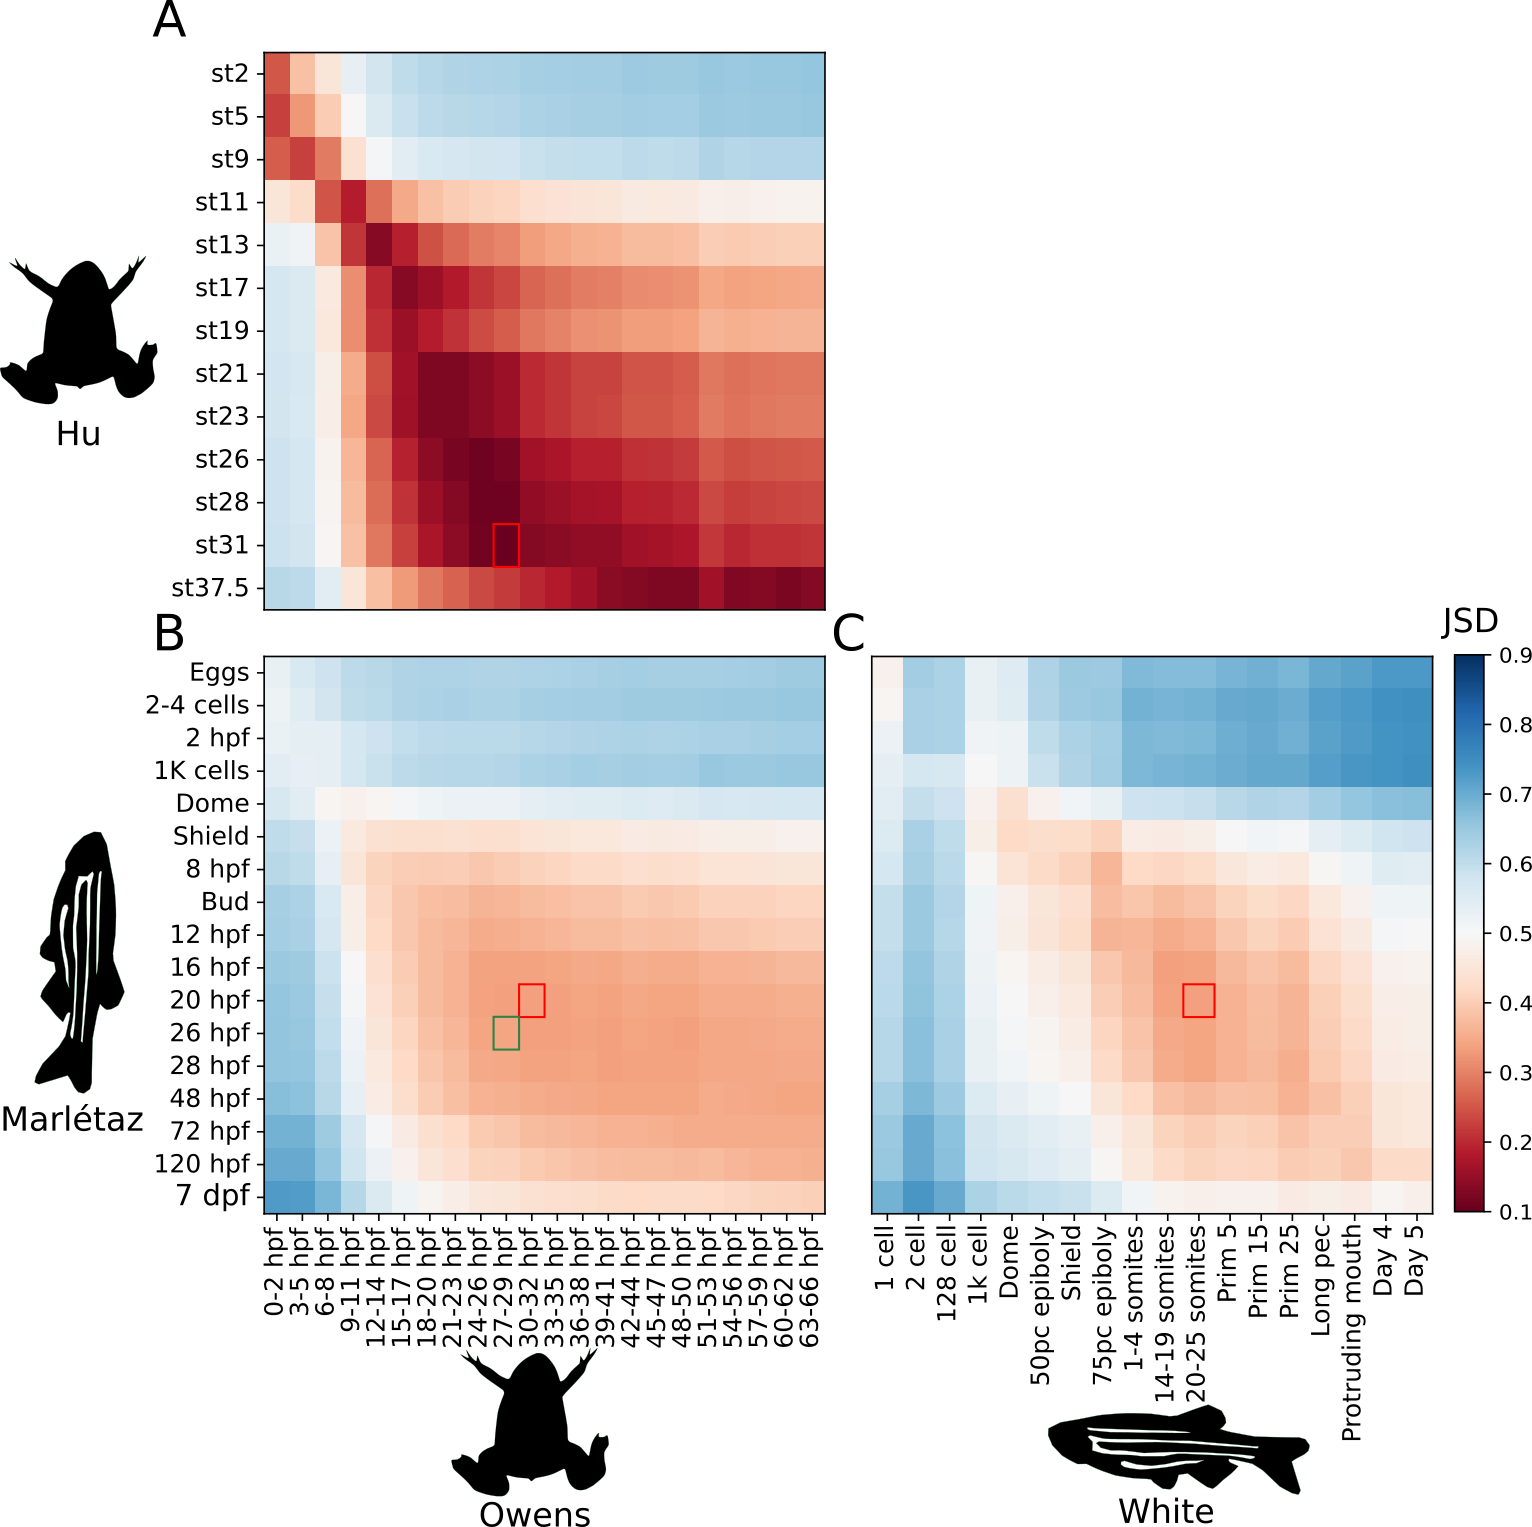
\includegraphics[width=\linewidth]{ch4.hourglass/images/between_experiment.png}
    \caption{Heatmap of pairwise Jensen-Shannon distances between (A) two \textit{Xenopus tropicalis} time series, (B) a \textit{Xenopus tropicalis} and a \textit{Danio rerio} time series, and (C) two \textit{Danio rerio} time series. The point of lowest Jensen-Shannon distance is marked in each comparison by a red square, and the green square represents the point of maximum similarity between \textit{Xenopus tropicalis} and \textit{Danio rerio} in the original study by Marl\'etaz et al.\cite{marletaz2018}.}
    \label{fig:betweenexperiment}
\end{figure}

Our re-analysis shows that an hourglass pattern already occurs in a within-species comparison. Any further comparison that is made between such time series suffers from this effect, and based on this basic re-analysis it is clear that the between-species comparison is just a superimposition of the two within-species patterns. How to correct for this effect NOT CLEAR and beyond the scope of this research, as there could be multiple explanations. The effect does not seem to be 

Still to write once finalized how we finish this:

\begin{enumerate}
    \item perhaps jensen shannon and highly expressed?
    \item not sure how to correct for it? Dividing JSD or subtracting, no clue what that means
    \item potentially works is subtracting euclidean distances, but best to leave that to real statistician + perhaps specifically generated data?
    \item we should show JSD between phyla. e.g. drosophila and c. elegans: point of max similarity happens at later time point, but time series also look quite bad.
    \item big difference zebrafish perhaps due to different sequencing protocols <-- important
    - strictly speaking between-experiment
\end{enumerate}

\subsection{The mid-developmental transition and the evolution of animal body plans} \label{subsection:levin}

In the paper \textit{The mid-developmental transition and the evolution of animal body plans} Levin \textit{et al.} compared the correlation coefficient of orthologous genes over time between ten species from different phyla. They found that most species-species comparisons had a high similarity in the beginning and a high similarity at the end of development, with a period of low similarity in the middle, which they called the \textit{mid-developmental transition}. They note that this period of low similarity between phyla seems to correspond to the phylotypic stage. They then suggest that this pattern could be used to distinguish different phyla. In this re-analysis, we demonstrate that we can find a \textit{mid-developmental transition} for both a within-phylum and between-phylum comparison. Moreover, we show that this pattern is a statistical artefact and can not be used to infer temporal conservational patterns.

Figure \ref{fig:within_phylum}A shows the pairwise Pearson correlation coefficient of one-to-one orthologs between each stage of \textit{Drosophila melanogaster} and \textit{Danio rerio}. With the same methodology of the original study we get a dual-phase pattern where both the early and the late stages between the two species seem conserved, but with a period of low conservation in the middle. If we now apply the same methodology to the chordates \textit{D. rerio} and \textit{X. tropicalis}, we get a similar biphasic pattern, indicating the \textit{mid-developmental transition} is not exclusive to between phyla comparisons. It is important to note that figure \ref{fig:within_phylum}B is based on the same count tables as figure \ref{fig:betweenexperiment}B. There are several minor differences in their processing, but the main reason for the large difference in trend is the gene standardization that is applied.

\begin{figure}[H]
    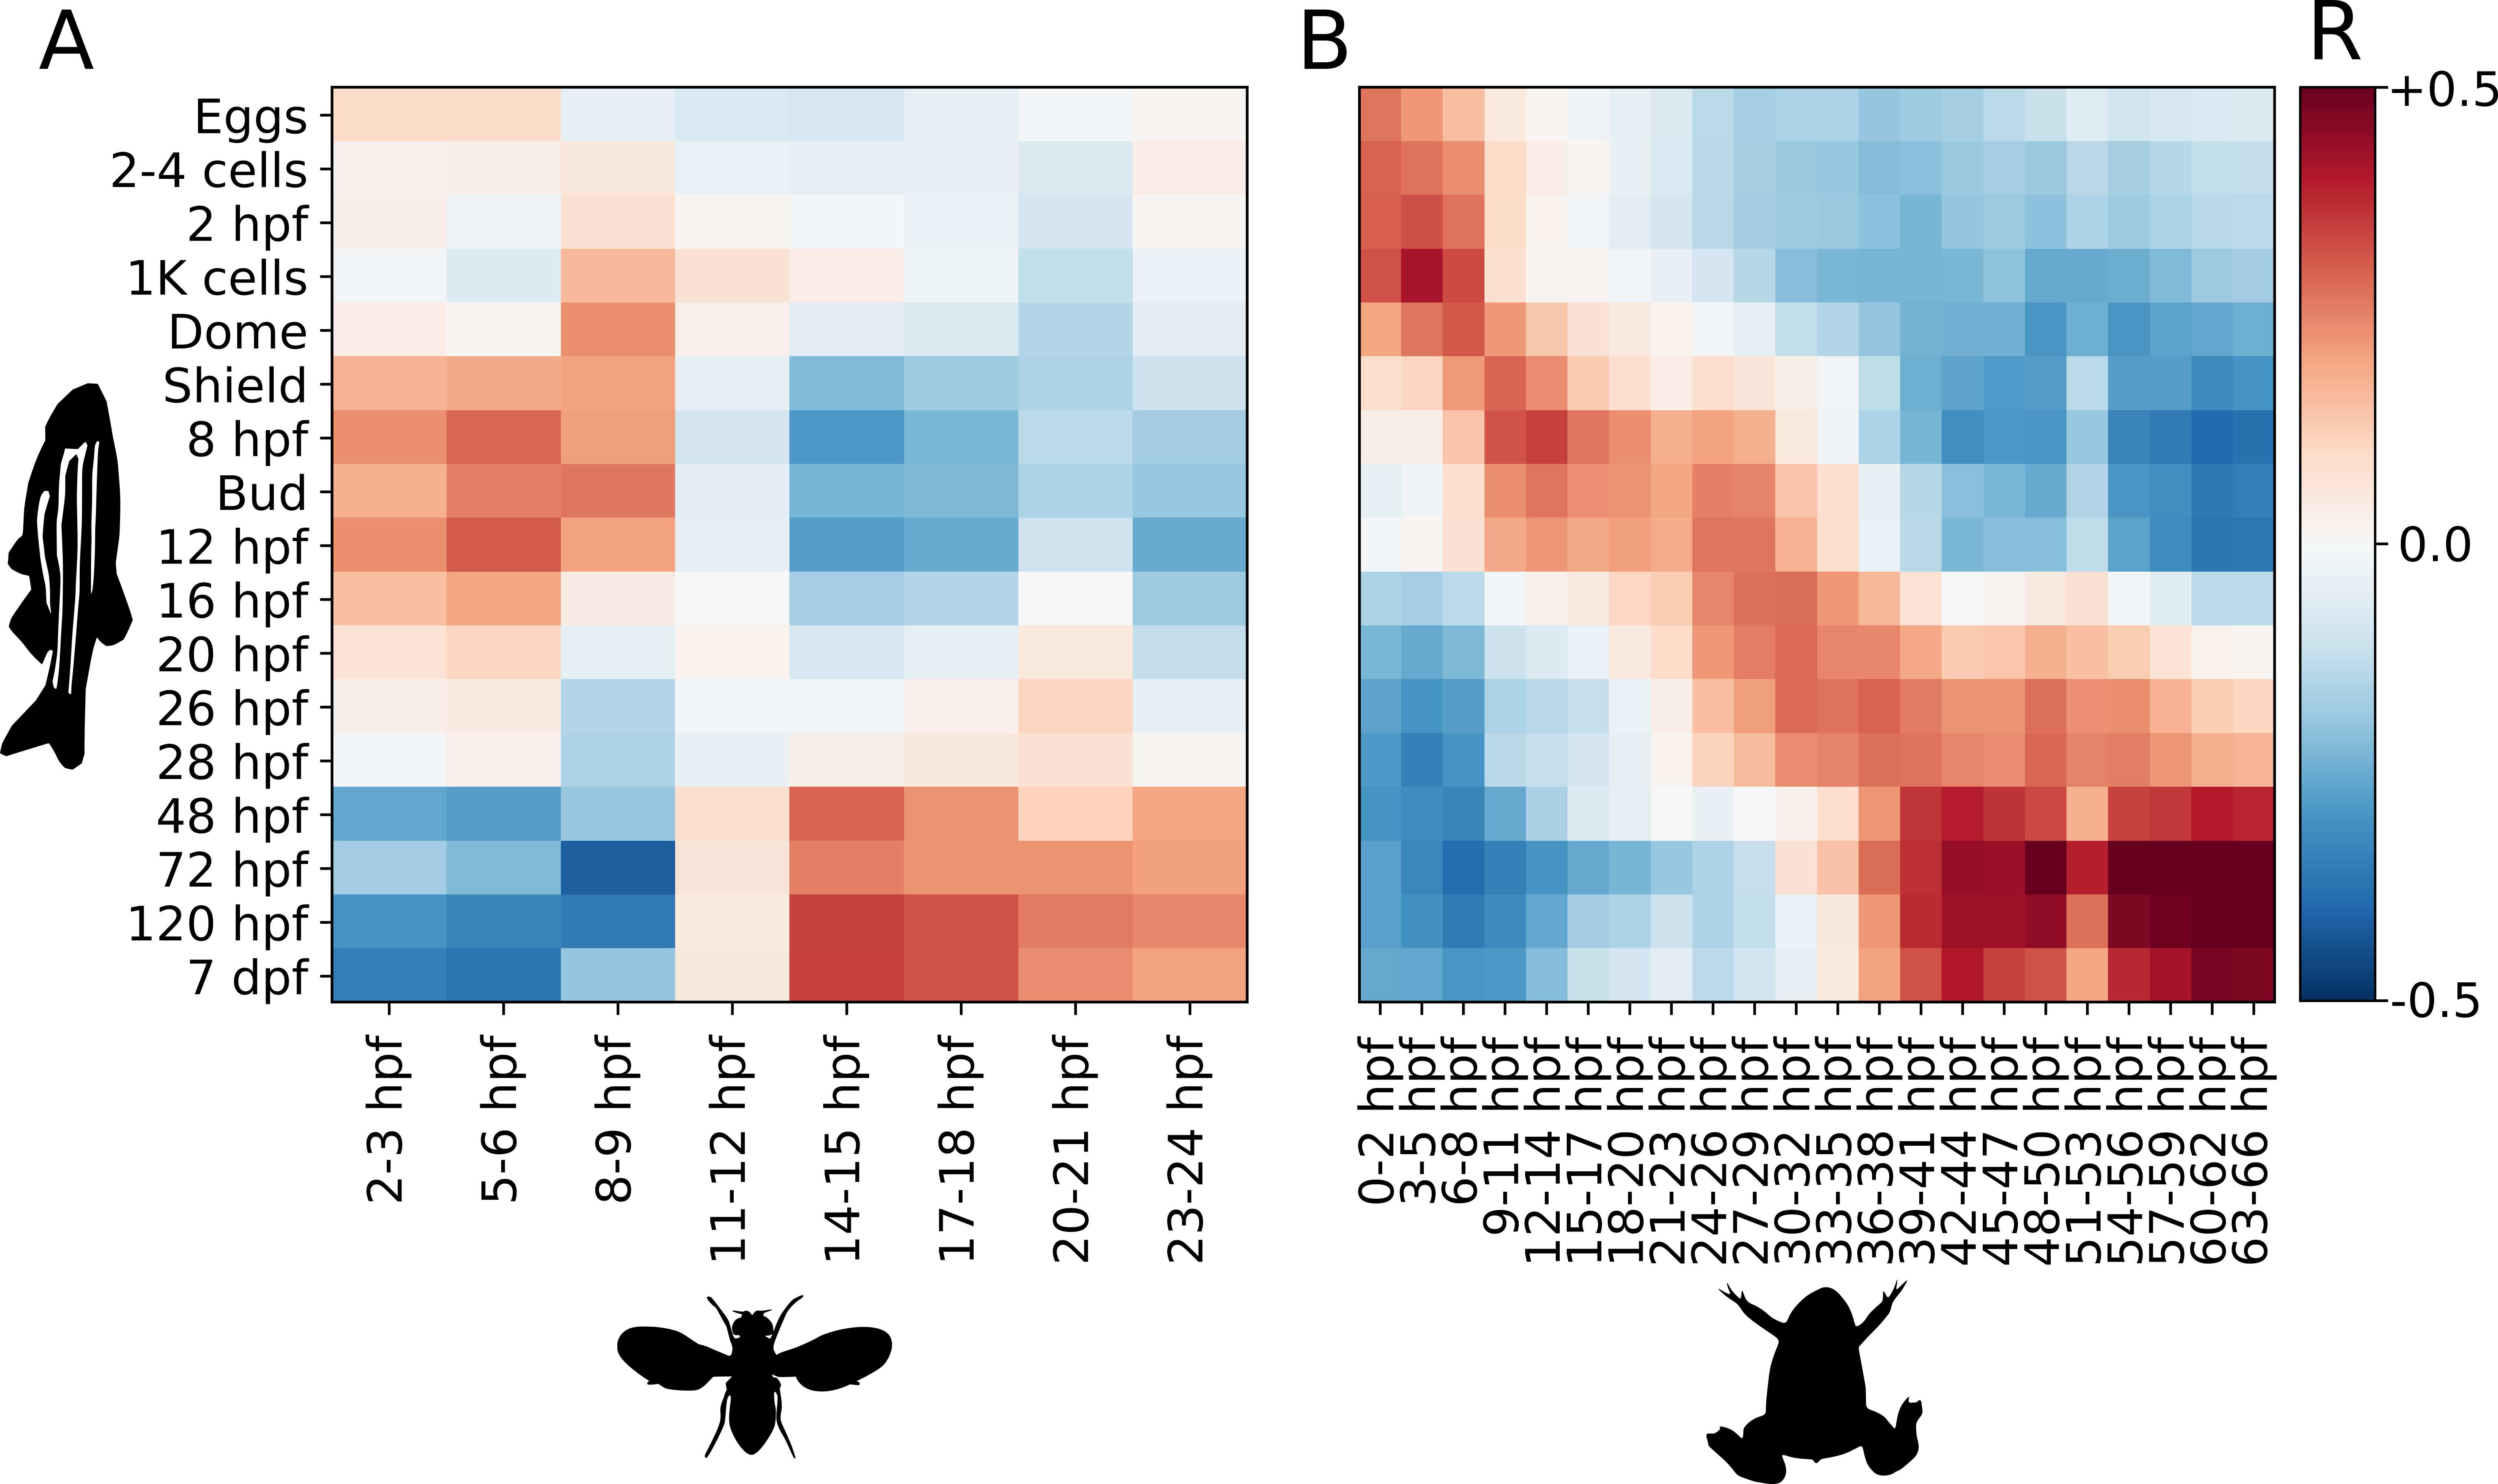
\includegraphics[width=\linewidth]{ch4.hourglass/images/within_between_phyla.png}
    \caption{Heatmap of pairwise Pearson correlation coefficients between (A) \textit{Danio rerio} and \textit{Drosophila melanogaster}, and (B) \textit{Danio rerio} and \textit{Xenopus tropicalis}. A mid-developmental transition occurs for both comparisons (between- and within-phyla).}
    \label{fig:within_phylum}
\end{figure}

Levin \textit{et al.} apply a standardization per gene. This means that each gene's counts have their mean over time subtracted and are divided by the gene's standard deviation over time. Standardization is generally a good practice for parametric methods like the Pearson correlation coefficient. In this case standardization effectively scales each gene to have equal weight in the correlation coefficient. If no standardization is applied, the extremes (the low and high expressed genes) have a higher importance in the calculation of the correlation coefficient than the rest of the genes. However, in our case standardization causes a surprising artefact. We can for instance cut each time series into halves, and after standardization, for three out of four comparisons still get a mid-developmental transition (fig. \ref{fig:normalisation}). 

\begin{figure}[H]
    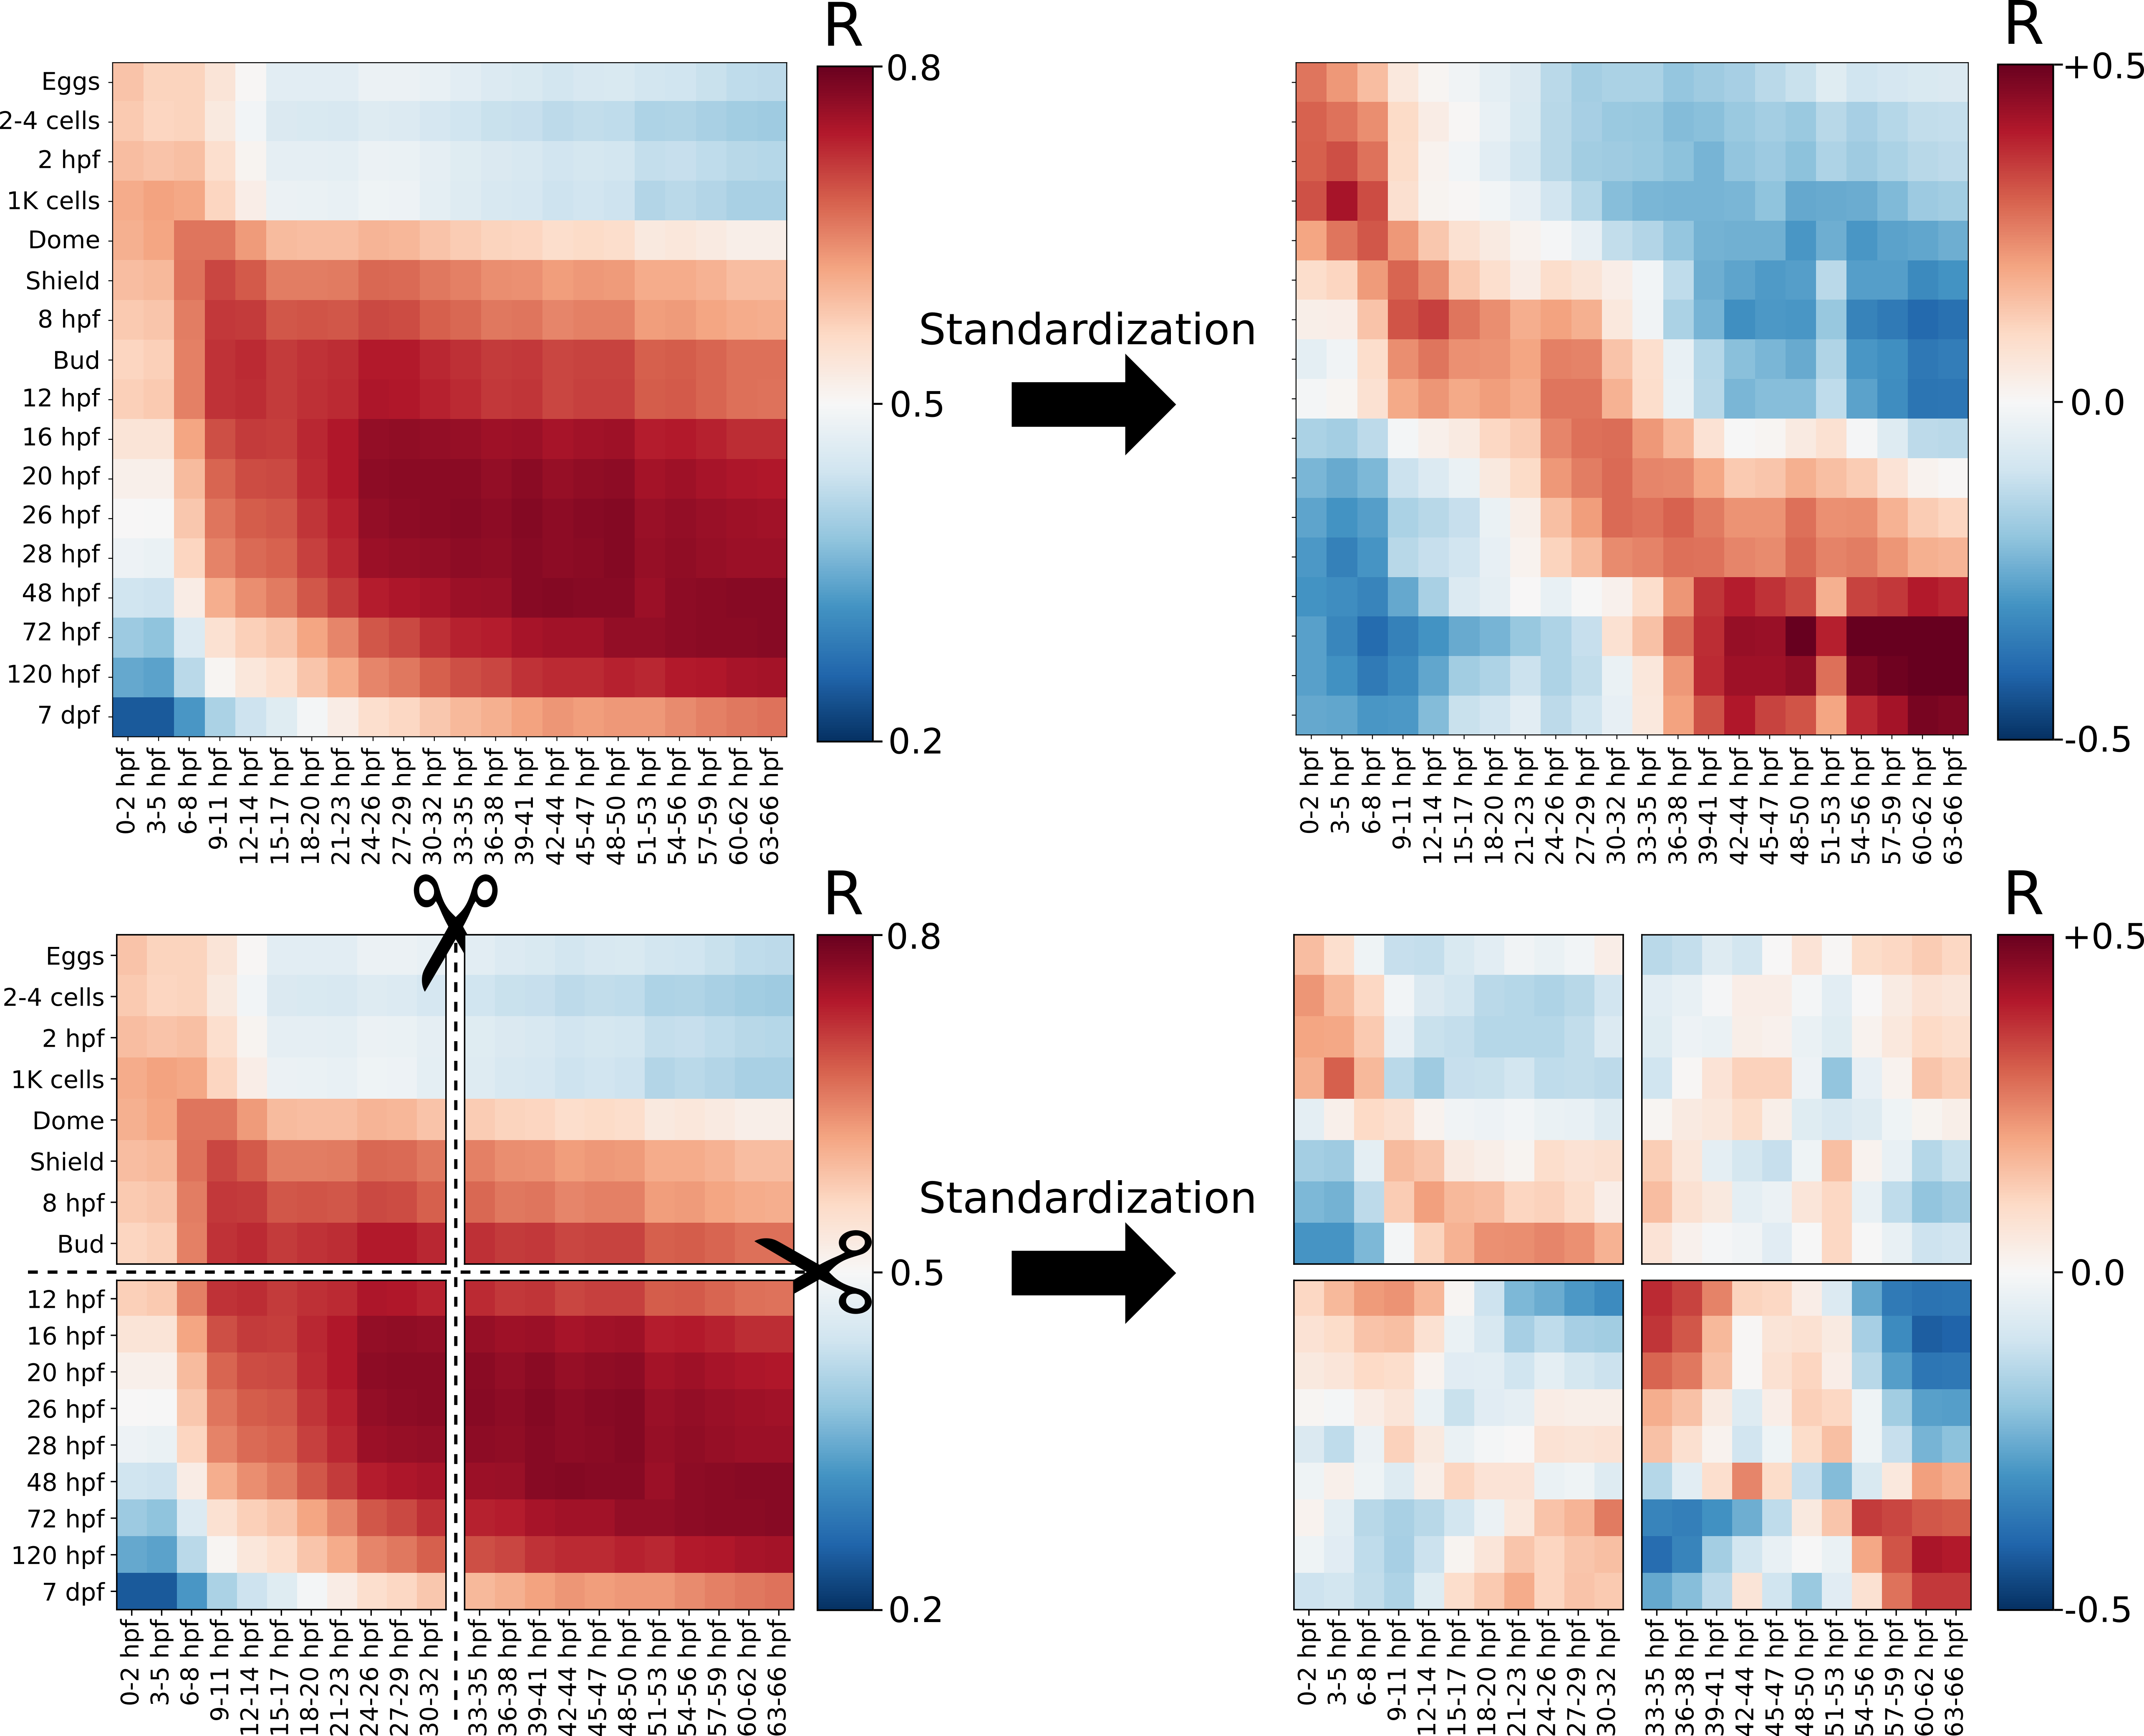
\includegraphics[width=\linewidth]{ch4.hourglass/images/normalisation.png}
    \caption{Heatmap of pairwise Pearson correlation coefficients which shows the effect of normalisation. The first image shows the not-normalised data, where each time series is cut in half. The second image shows the effect of normalisation on pairwise Pearson correlation coefficients. Whereas the original data had a point of maximum similarity approximately in the middle of the time series, three out of four subsets now show an inverse hourglass. TODO NEEDS AN A AND A B}
    \label{fig:normalisation}
\end{figure}

To get an understanding as to why this happens we need to study the patterns of gene expression during development. Similarly to Levin \textit{et al.}, we've calculated the Pearson correlation coefficient for each gene with a linearly increasing line (this is what Levin \textit{et al.} call the gene landscape in their study). A coefficient of 1 would mean that a gene is linearly going up over time, a coefficient of -1 would mean that a gene is linearly going down over time, and a coefficient of 0 would mean that a gene shows no temporal pattern. In figure \ref{fig:genelandscape} we show the histogram of Pearson correlation coefficients for \textit{D. rerio}, \textit{D. melanogaster}, and \textit{X. tropicalis} per gene over time. For each comparison we get an arc, with an enrichment for genes that are either going up or down over time, with relatively few genes having no temporal pattern. The scatterplot of Levin \textit{et al.} unfortunately hides this pattern, and a 2d histogram would have been a better choice. The explanation for as to why we get this pattern is actually pretty straightforward. Most embryos grow extensively during development, and as the embryo grows we expect the total amount of mRNA to increase as well. But, most sequencing protocols quantify a fixed amount of transcripts per sample, which means that the total of measured transcripts stays constant over time. This effectively means that genes get split into either one of two expression groups; a group where gene expression increases faster than the average gene (right side of the gene landscape), or the group where gene expression increases slower than the average gene(left side of the gene landscape). This also explains why this pattern is less pronounced for \textit{D. melanogaster}, as this embryo grows little in size during development. See figure \ref{fig:genelandscapenormalization} for the difference between per-embryo normalization and transcript per million (TPM) normalization for \textit{X. tropicalis} embryos.  

\begin{figure}[H]
    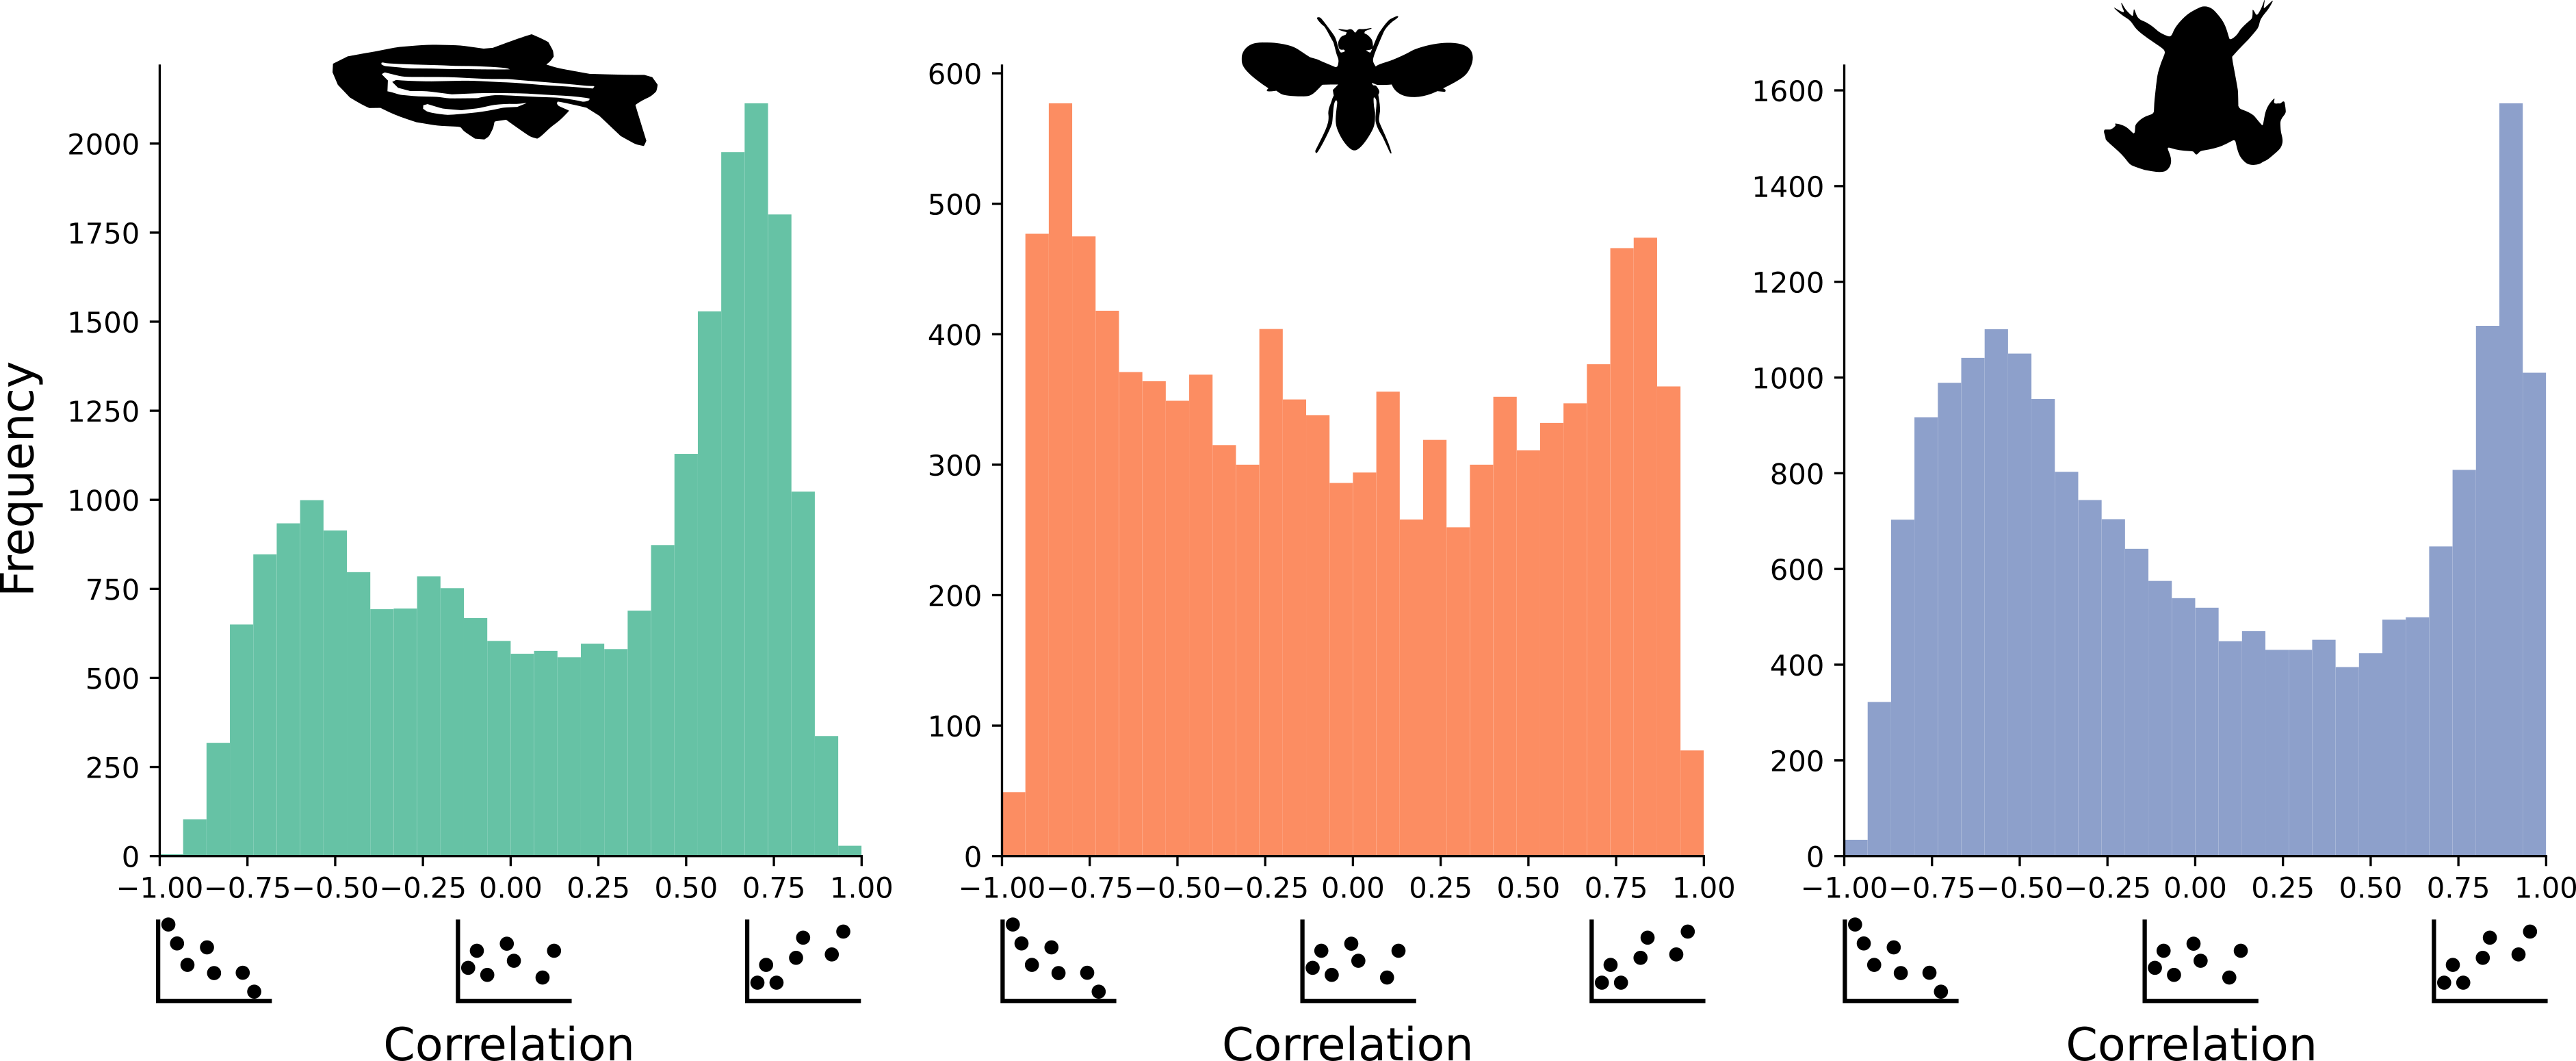
\includegraphics[width=\linewidth]{ch4.hourglass/images/gene_landscape.png}
    \caption{gene landscape TODO}
    \label{fig:genelandscape}
\end{figure}

Now that we know that our genes can be classified as either going up or going down over time, we can think about how this influences our analysis. Let's start by imagining the time-series of a single gene which has a binary expression profile, where at the start of our time-series the gene is \textit{off}, and at a random time point switches \textit{on} and stays on until the end of the series. We now imagine the expression profile of this gene in a related species, and assume again that it starts \textit{off} and at random time point switches \textit{on}. We can express the probability that these two imaginary time-series are equal (section \ref{subsection:middevelopmenttransition}), and if we visualize these probabilities it is clear these odds show a mid-developmental transition (fig. \ref{fig:inverse_math}). This theoretical derivation is a however an extreme oversimplification of what happens biologically and considers only a single gene. For this reason we simulated two time-series with a continuous expression profile. In these series half of the genes start in an \textit{off} stage where expression is zero, and half in an \textbf{on} where expression is one. Similarly as the thought experiment, these genes, at a random time-point, gradually switch from \textit{off} to \textit{on}, or vice versa (fig. \ref{fig:sim_explanation}A). We can now calculate the Pearson correlation coefficient between these simulated series, and again we get a clear mid-developmental transition. Similar to the biological data, if we cut the simulated data into halves, and apply standardization afterwards, we get a mid-developmental transition per subset of the data (fig. \ref{fig:sim_normalisation}). 

\begin{figure}[H]
    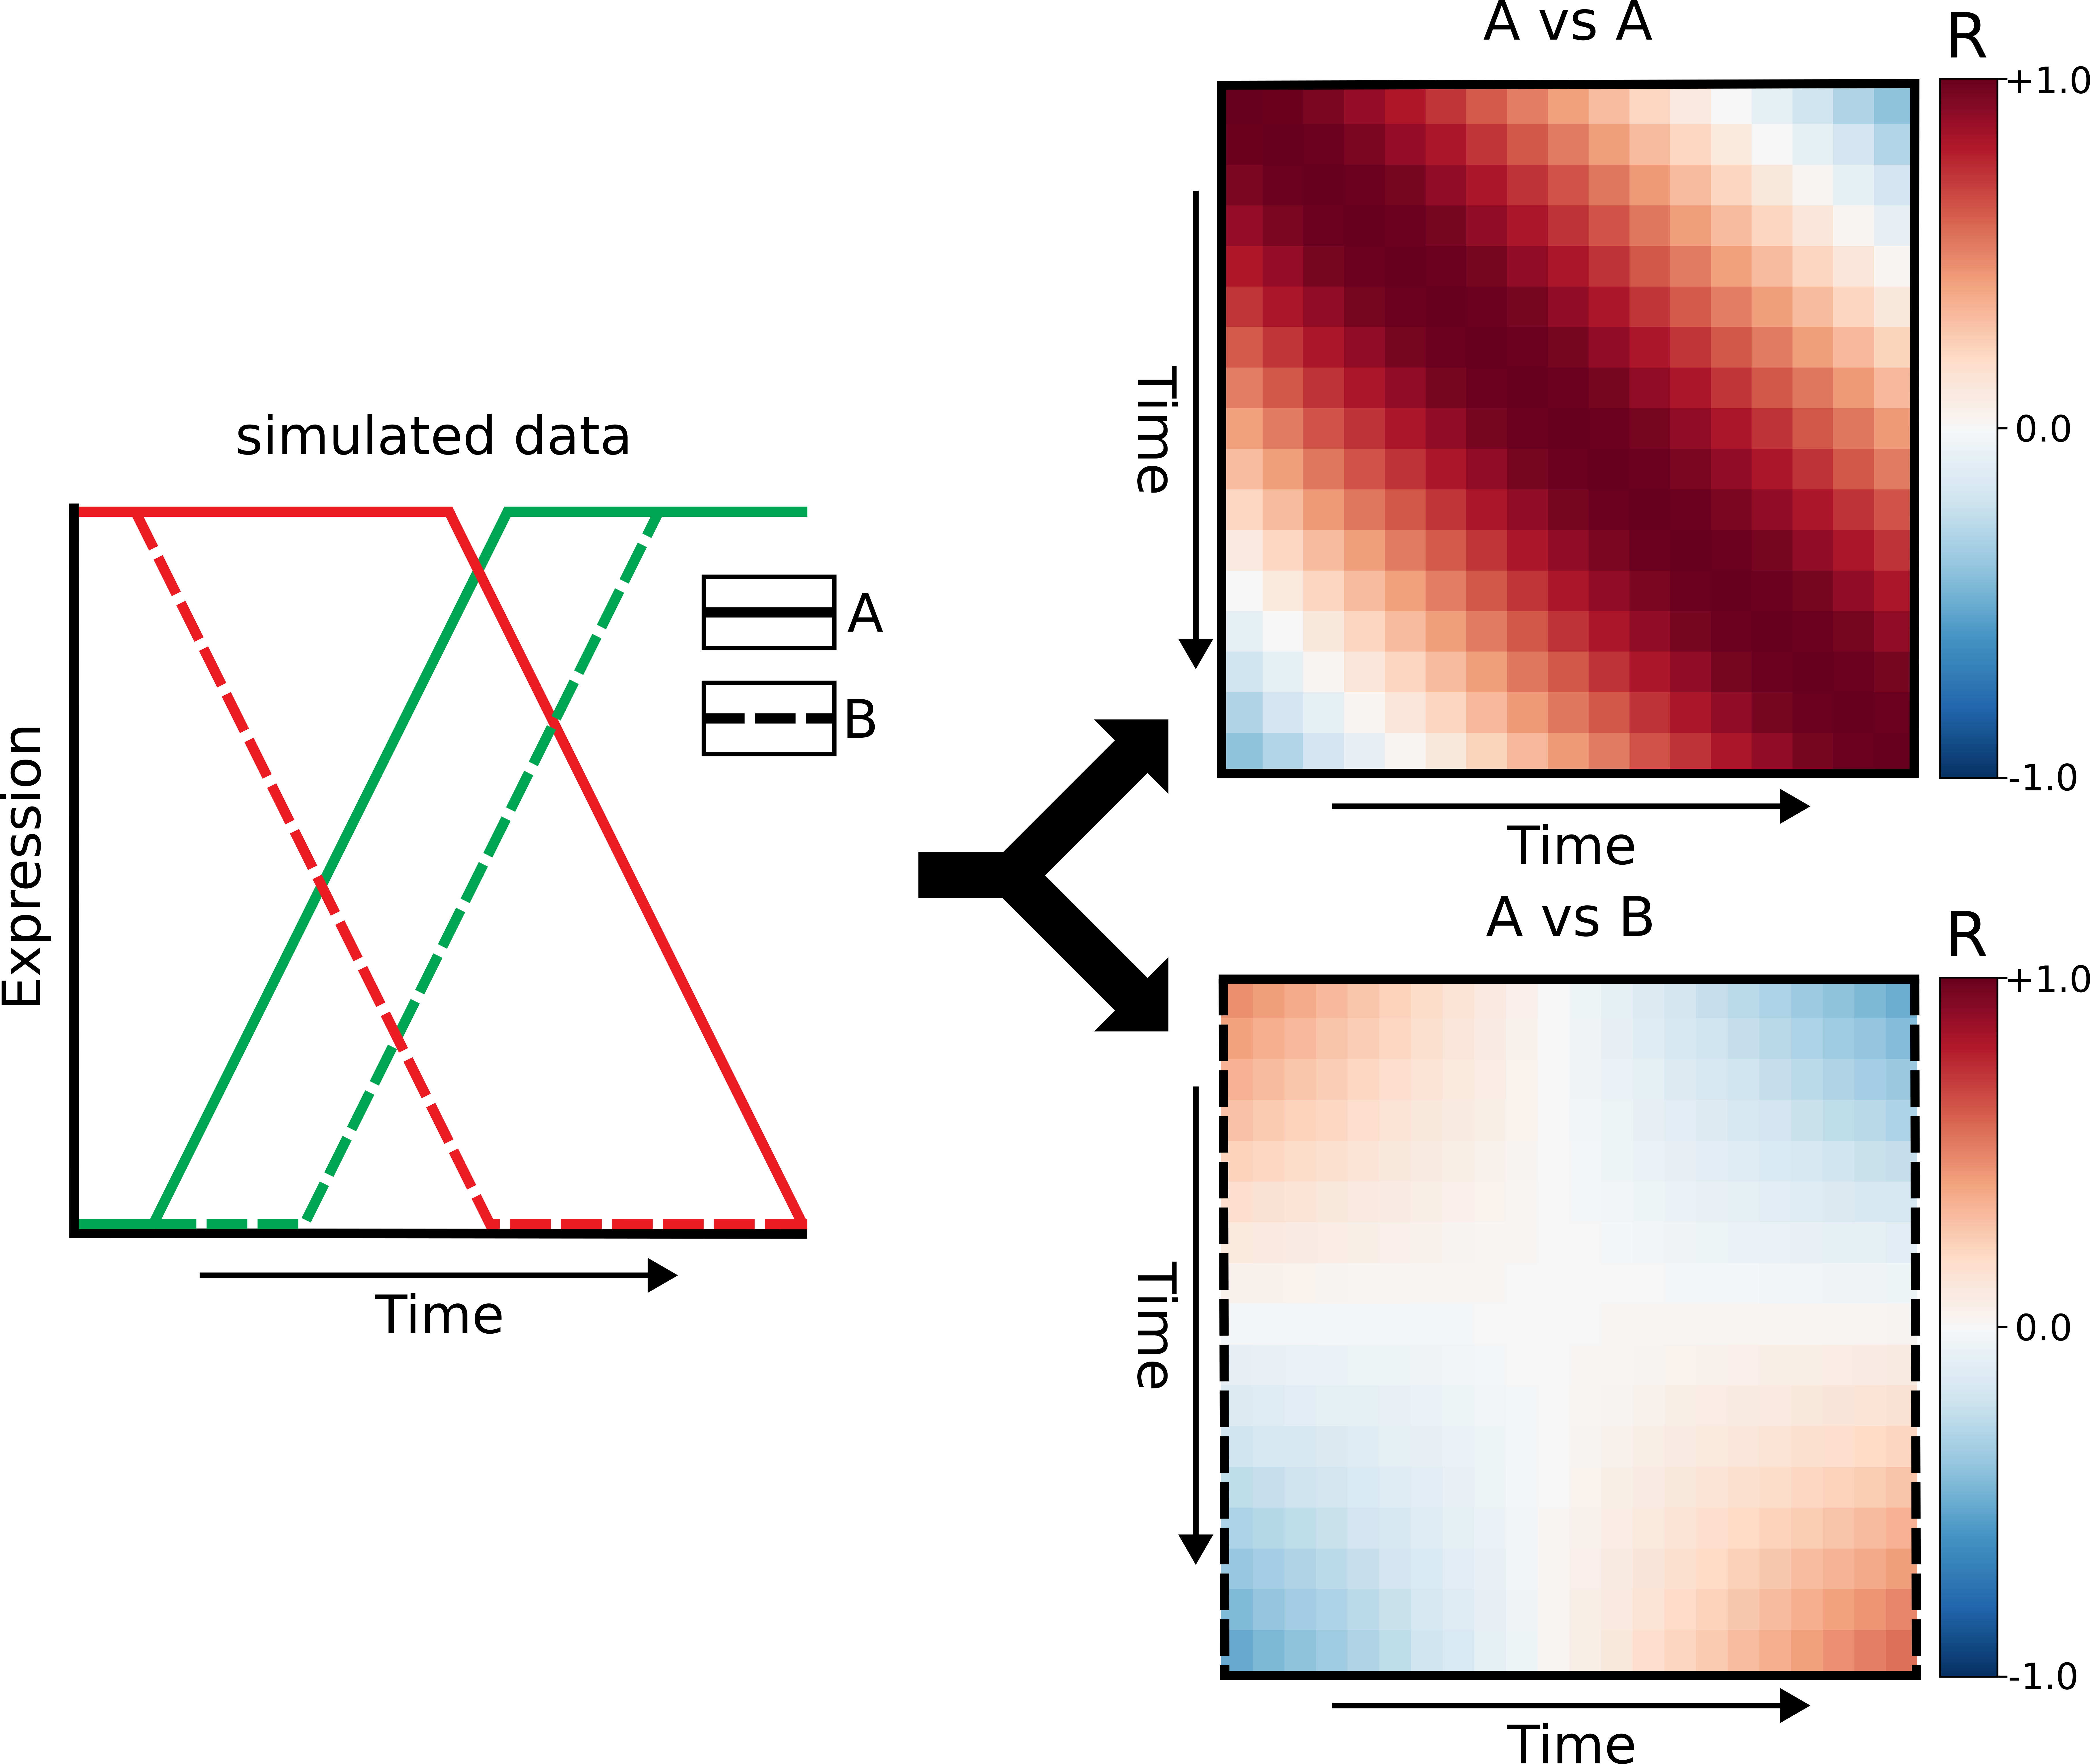
\includegraphics[width=\linewidth]{ch4.hourglass/images/sim_explanation.png}
    \caption{TODO explanation.}
    \label{fig:sim_explanation}
\end{figure}

By incorporating a within-phylum comparison it becomes clear that the mid-developmental transition is a statistical artefact of gene standardization. It can be considered a case of Simpson's paradox, where by standardization gene expression gets put into two groups (high vs low expression). Where there is no particular correlation within each group, but with a clear correlation when comparing the data set as a whole\cite{Saccenti2023}. It is important to note that we've applied the same criteria as Levin \textit{et al.} to only include dynamic genes (minimum expression of 10 and at least a log2 fold change). This means that this pattern is not caused by irrelevant and lowly expressed genes. As such we see no molecular basis for an inverse hourglass model between phyla, which leaves the question as to how the phylotypic stage behaves in comparisons between-phyla wide-open.

\subsection{The hourglass model of evolutionary conservation during embryogenesis extends to developmental enhancers with signatures of positive selection} \label{subsection:liu}

In the paper \textit{The hourglass model of evolutionary conservation during embryogenesis extends to developmental enhancers with signatures of positive selection} Liu \textit{et al.} compare the similarity of accessible regions over five matched embryonic developmental time points between two \textit{Drosophila} species (\textit{D. melanogaster} and \textit{D. virilis}). Liu \textit{et al.} find that the middle time point (TP3) uses the most enhancers, and is the most conserved between these two flies (figure \ref{fig:peak_null}B). In this re-analysis we show that this hourglass pattern can simply be explained by the different number of enhancer regions found per time point.

In this study conservation is defined as the similarity between time point specific enhancers between \textit{D. melanogaster} and \textit{D. virilis}. Time point specific enhancers are defined as enhancers that are enriched in only one time point (TP), and similarity is calculated by dividing the number of TP-specific enhancers that are enriched in both species for the same time point with the number of remaining TP-specific enhancers for that time point(Jaccard index). Figure \ref{fig:peak_null}A shows the Jaccard index per time point between \textit{D. melanogaster} and \textit{D. virilis}, with the highest value at TP3, the \textit{Drosophila} phylotypic period\cite{Liu2021}. If we apply the same methodology between replicates from \textit{D. virilis}, we get a different pattern, where TP1, TP3, and TP5 are most conserved between replicates of the same species(fig. \ref{fig:peak_null}C). This pattern between replicates indicates a potential bias in the analysis. Upon inspection it seems that the number of TP-specific enhancers seem positively correlation with the Jaccard index(fig. \ref{fig:peak_null}B,D). To test whether this relation exists we've made a consensus set of enhancers over all the time points, and assign each time point a set of randomly picked enhancers, while keeping the number of enhancers per time point the same as originally found \ref{fig:shuffle}A. This removes all biological meaning from the data, but yet, still shows the highest Jaccard index at TP3 between species. The obvious way to control for this would be to subsample all time points to the same number of peaks \ref{fig:shuffle}B. Once subsampled, we find that TP2 shows the highest conservation between enhancers between \textit{D. melanogaster} and \textit{D. virilis}. The dependence of the Jaccard index on the number of enhancers can also be formally proven, see section \ref{subsection:flypeaks}. 

\begin{figure}[H]
    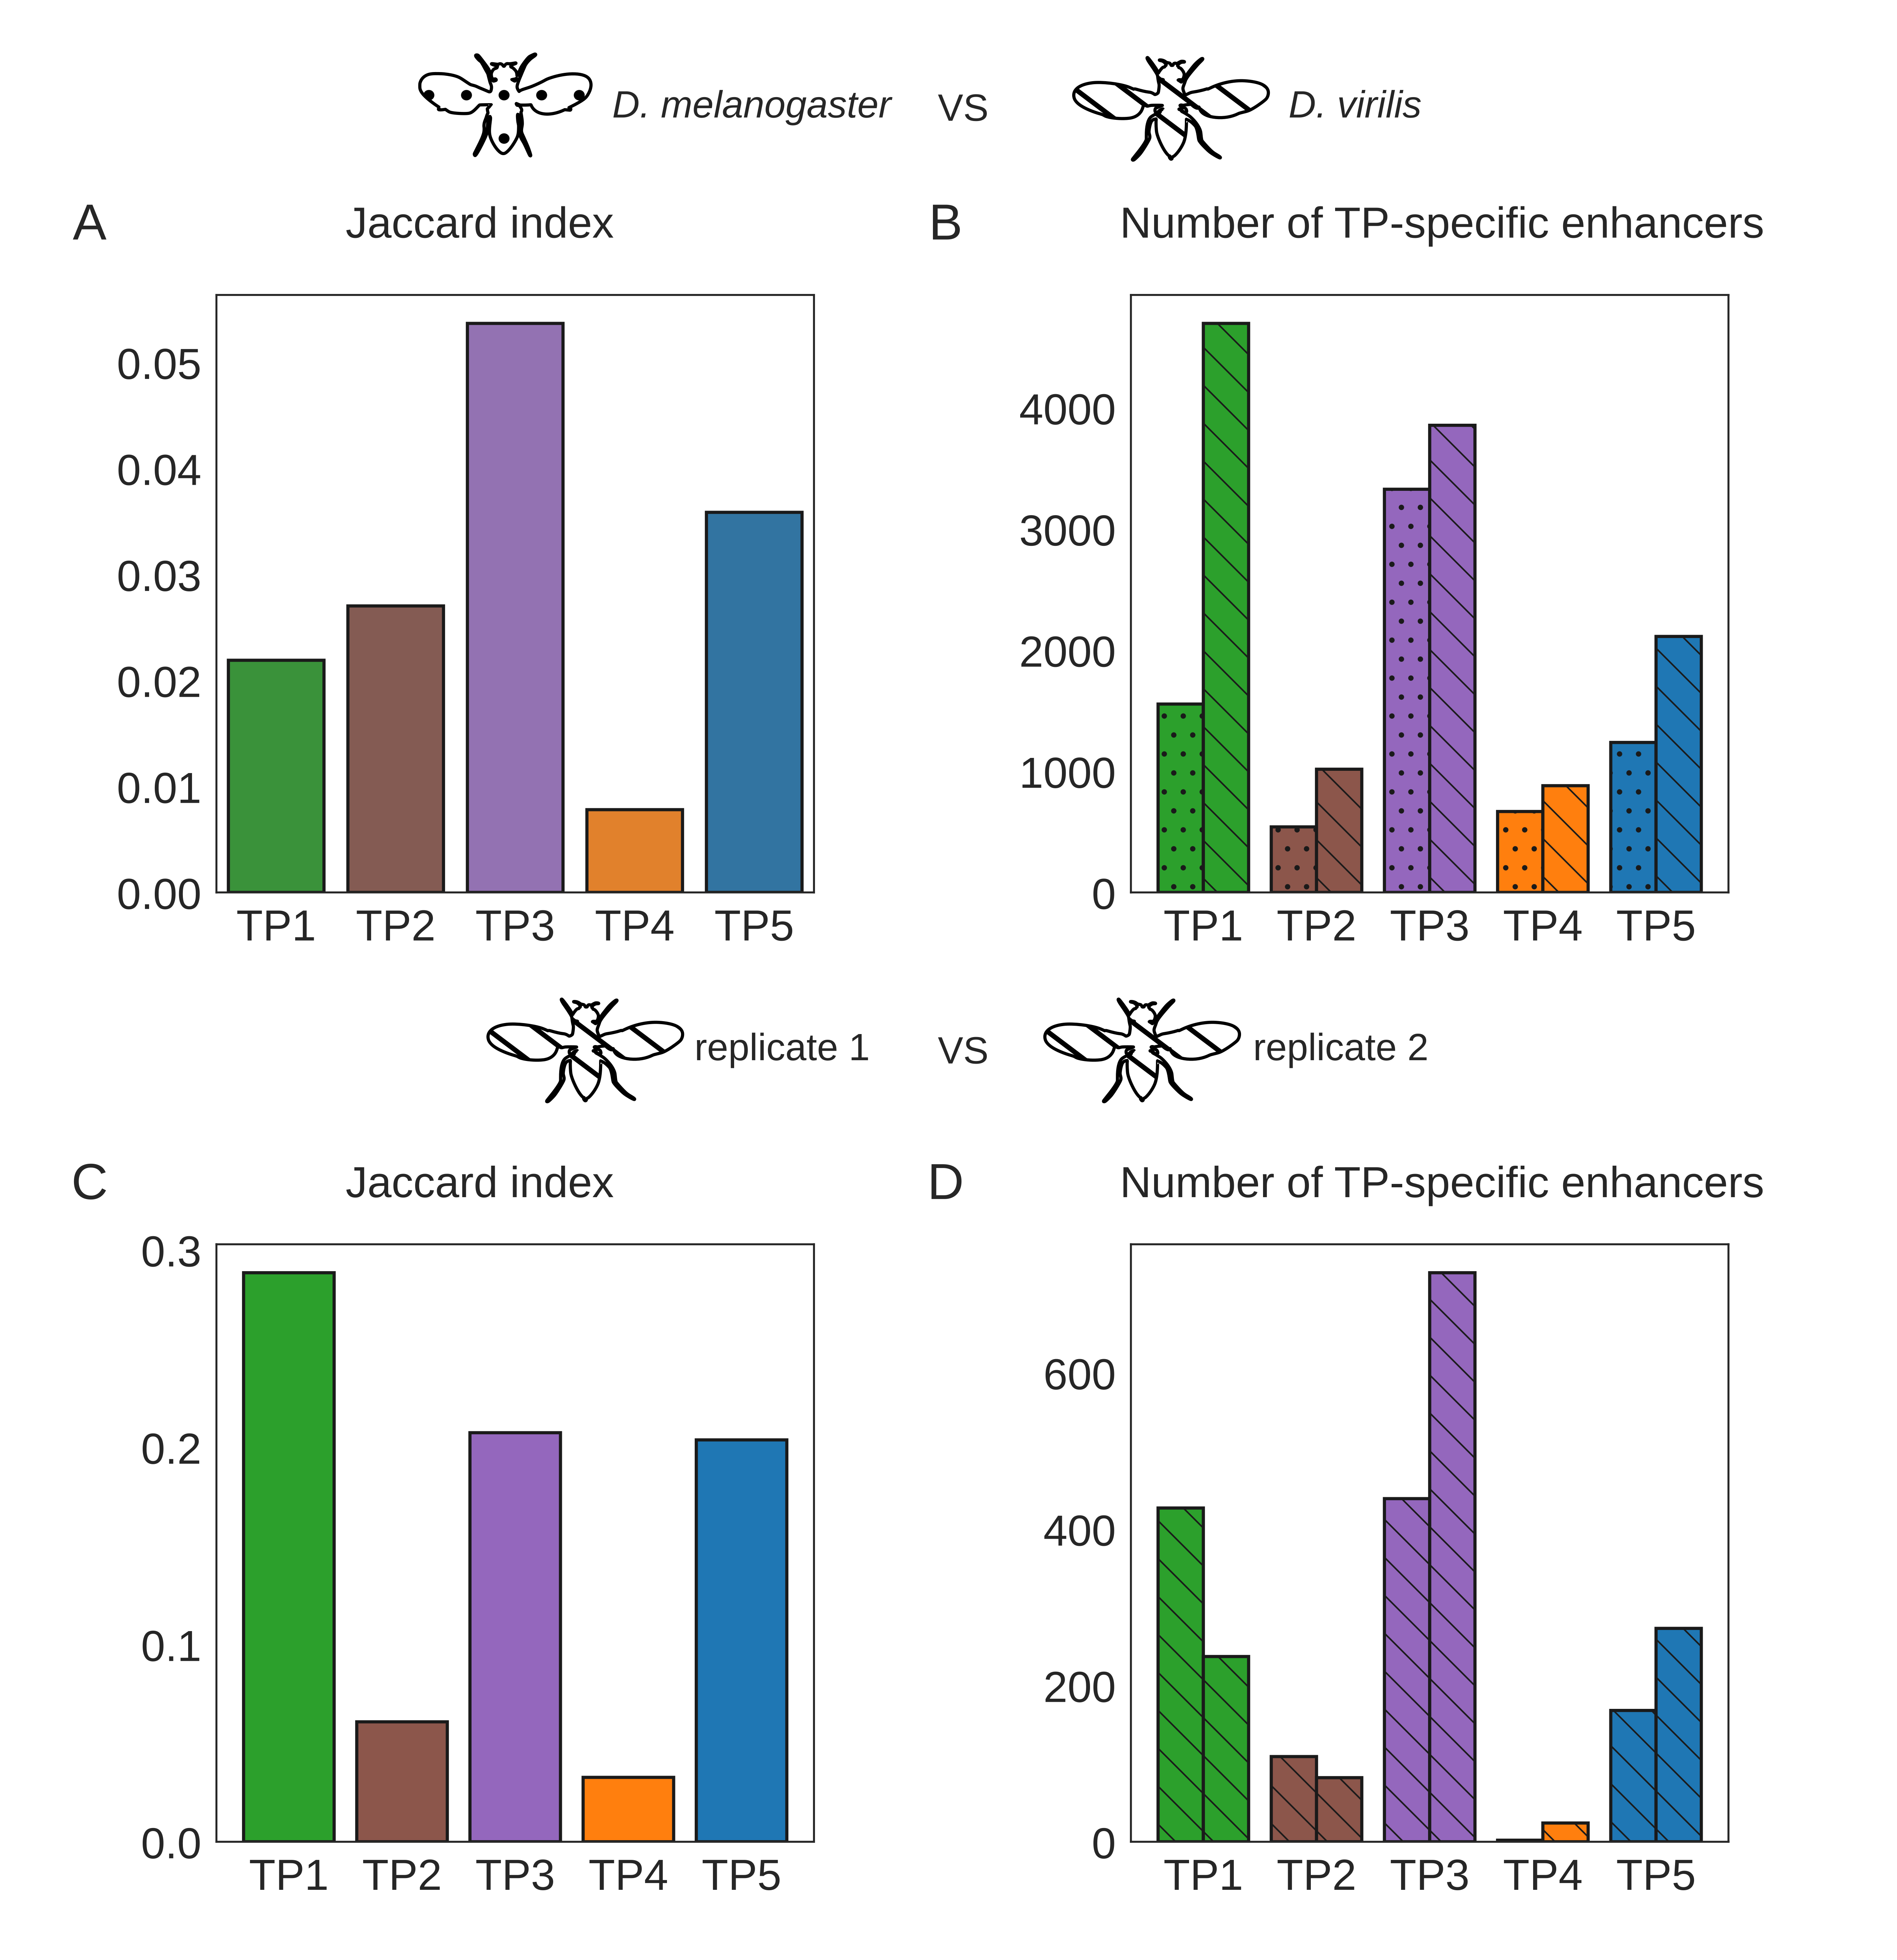
\includegraphics[width=\linewidth]{ch4.hourglass/images/fly_control_2.png}
    \caption{TODO. melanogaster vs virilis and rep1 vs rep2. Jaccard index and number of enhancers}
    \label{fig:peak_null}
\end{figure}

\begin{figure}[H]
    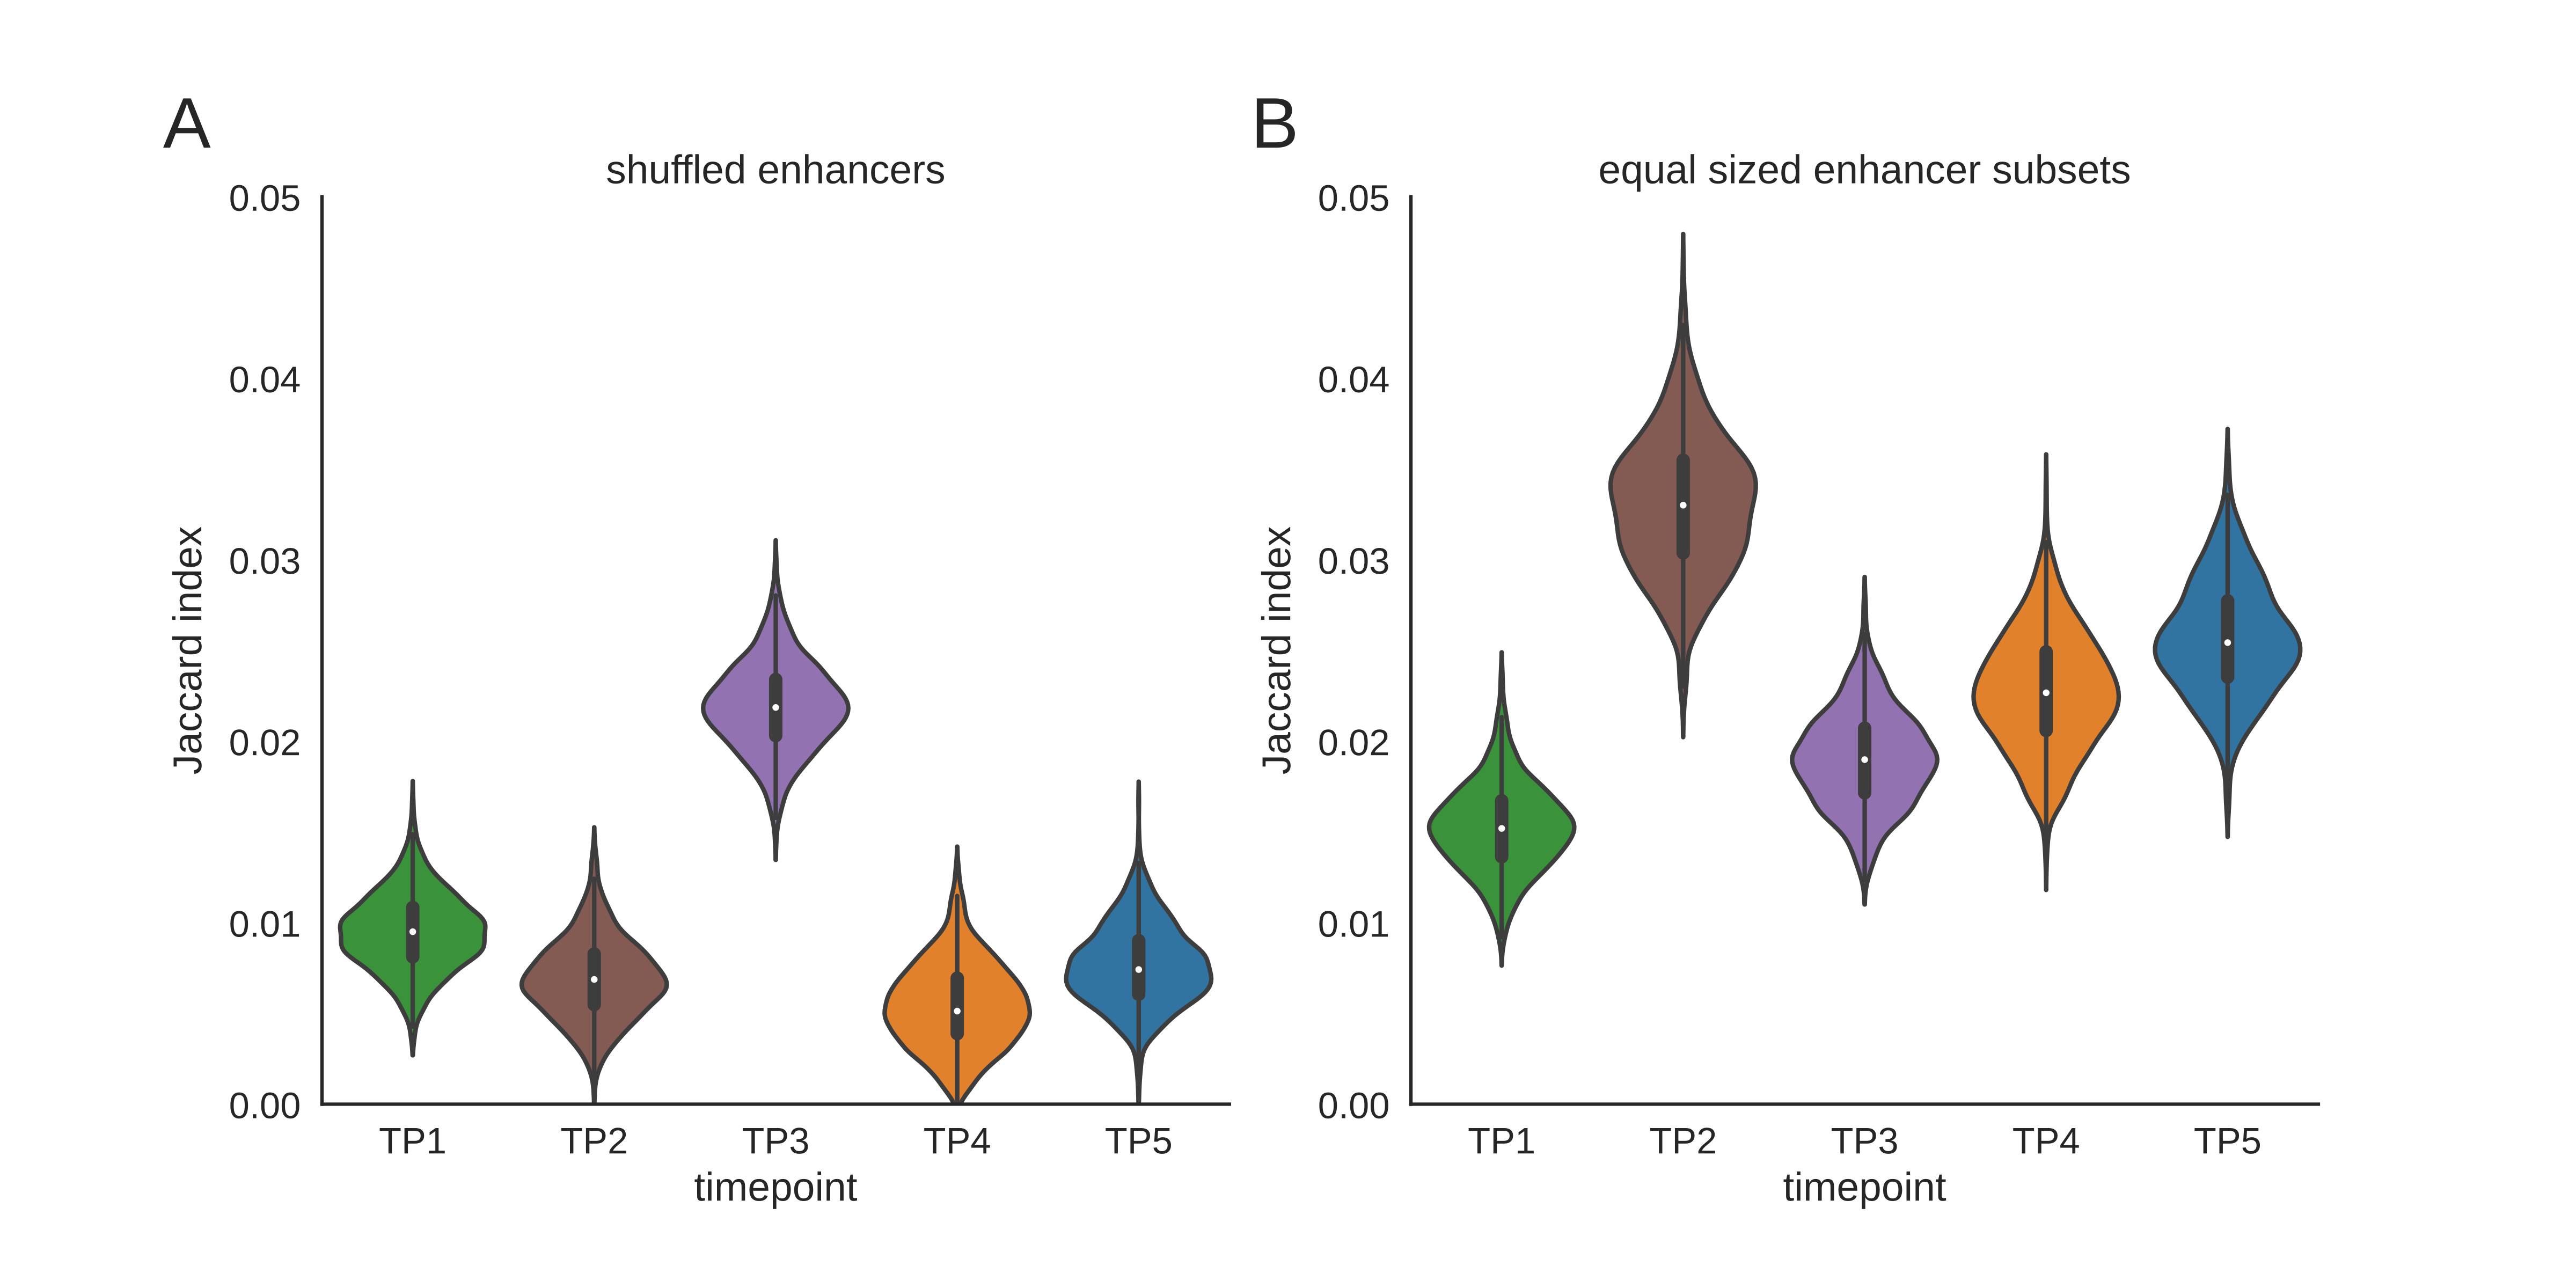
\includegraphics[width=\linewidth]{ch4.hourglass/images/fly_shuffle.png}
    \caption{shuffle explanation.}
    \label{fig:shuffle}
\end{figure}

Apart from a biological interpretation for the different number of time-point specific enhancers, there are also two methodological interpretations. Firstly, the focus on TP-specific enhancers creates artificial sets of TP-specific enhancers. TP-specific enhancers are defined as occurring in one time-point only. This means that if two time-points are sampled more closely in time than other time-points, these two time-points would share most of their enhancers, resulting in a low number of TP-specific enhancers, something the authors themselves already note. Similarly, enhancers at the beginning and the end of the time-series have a higher chance of being TP-specific purely because they are only compared against one adjacent time-point whilst the rest of the time-series are compared against two. The percentage of reads in the consensus peak set in enhancers vs promoters per time point for instance shows no clear enrichment for a specific time-point (fig. \ref{fig:peak_enrichment}). Secondly, during peak calling arbitrary thresholds are used to decide whether a region is \textit{enriched}. This threshold depends for instance on the signal-to-noise ratio, which is expected to change for a developing embryo, and the sequencing depth\cite{encode_guidelines2012}. Which neither of them have been corrected for in the original analysis.

Moreover, Liu \textit{et al.} proceed to train a computational model on the sequences of time-point specific enhancers of \textit{Drosophila melanogaster}. This model is then used to classify enhancers for whether they are subjected to positive selection. They then find that the ratio of enhancers subjected to positive selection vs enhancers subjected to non-positive selection is high for TP1, TP3, and TP5, and thus conclude that the molecular basis for the phylotypic stage can partially be explained by positive selection of gene regulation conservation. We would argue instead that there are again two likely methodological explanations to this pattern. The first explanation is that as there has been no correction for signal-to-noise ratio and sequencing depth, there is a difference in the type(s) of peaks the pre-processing picked up, which in turn translates to different predicted positive selection ratios. The second explanation is that, as is true for practically all machine learning, the model generalizes and performs better with more training data. Looking at their reported model performance (AUC) we can clearly see that the model's performance for TP1, TP3, and TP5 is notably higher than for TP2 and TP4. Looking back at figure \ref{fig:peak_null}D we see that the high model performance closely follows to the amount of training data (number of TP-specific peaks). This could simply mean that \textit{better} trained models predict a higher amount of positive selection. Without correction for these potential confounders it is hard to reach a definitive conclusion about positive selection with regards to the hourglass model and the phylotypic stage.

By comparing the within-species conservational pattern we expose important flaws in the experimental design of this study. Our re-analysis shows that the fact TP3 seems highest conserved between \textit{D. melanogaster} and \textit{D. virilis} is an effect of the number of TP-specific enhancers, and not because this time point is more conserved between these two species. Moreover it seems that the number of TP-specific enhancers also influences the downstream training of the gkm-SVM and in turn the pattern of enhancer positive selection. 

\section{Discussion}

Our study highlights the importance of including within-species, within-phylum and between-phylum comparisons in the analysis of the phylotypic stage. We demonstrate that the high transcriptome similarity between \textit{D. rerio} and \textit{X. tropicalis} at the phylotypic stage can be explained by within-species effects alone. Furthermore, we identify the mid-developmental transition and \textit{Drosophila} enhancer conservation at the phylotypic stage as statistical artefacts. 

When comparing time-series directly, it is important to control for statistical biases in the data, such as the correspondence between replicates, but also the temporal sampling strategy, data distribution, cell type proportion and gene sets used. A key bias that is often overlooked is whether the sampling schema follows developmental time\cite{BinindaEmonds2002}. It is not uncommon for studies to report a discontinuous blocked pattern of within-species conservation, where the difference between stages is not equal. This difference often gets assigned a biological explanation; for instance as embryonic genome activation\cite{Yanai2011} or developmental milestones\cite{Levin2012}. However, this blocked within-species pattern proceeds to affect the between-species comparison where the same blocks are visible. From a data science point of view, the only way to make a fair comparison between time series is when the similarity between all adjacent time points is equal (or if one explicitly corrects for this bias statistically). When sampling stages closely in time, one increases the probability of stages to match closely in a comparison with another time-series. This in turn increases the expected maximum similarity. The reverse is also true, where stages sampled in large intervals reduces the probability of matching stages between time-series, which then reduces the expected maximum similarity. Thus under the assumption that embryonic development has no point of higher selective pressure, a comparison between two time-series will have the highest expected similarity at the point where sampling has happened at the shortest interval. For this reason we argue for a re-definition of molecular embryonic time, where not morphological features or time post fertilisation is used, but where the (molecular) difference between adjacent stages is equal.

Similarly, changing gene expression distributions are an effect of developmental maturity\cite{Kannan2021}. Pluripotent tissues have relatively many genes activated, whilst more mature tissues make use of a smaller more specialized set of genes. These changing gene expression distributions over time can introduce unexpected biases and artefacts when calculating similarity. For instance, the JSD and Pearson correlation coefficient between two count tables from different distributions can respectively never be zero or one. As an effect, directly comparing similarity scores between time-points can be misleading as the range of possible similarity scores is different per comparison. To circumvent this problem one can resort to non-parametric distance metrics, such as the rank-based Spearman correlation coefficient\cite{Irie2011}, or quantile normalizing the data before calculating the distance metric\cite{marletaz2018}. Then, one can compare the similarity scores directly, but these approaches ignore the biologically relevant gene expression distribution changes. As long as there is no consensus on what type of molecular similarity is expected at the phylotypic stage, it can both be correct as well as incorrect to ignore the distributional changes. 

Another point to consider is the changing proportions of cell types. An embryo is formed by all the multiplying and developing cells together, and their combined signal is measured in the study of the molecular phylotypic stage. But not every cell type expresses the same amount of transcripts\cite{Kim2023, Percharde2017}, which consequently gives cells with a lot of transcripts a higher importance in the (dis)similarity calculation. Moreover, changes in similarity between species could be either caused by changes in gene expression, or by changes in cell proportions. For example, during the vertebrate phylotypic stage the neural tissue is already highly developed and relatively large. Perhaps similarity at the vertebrate phylotypic stage is an effect of the over-representation of these neural cell types. Or as another example, a practically universal feature of embryos is that they grow during development. But because of this growth, for example, the surface (skin) to volume (organs) ratio changes, which could be another driving force for the molecular phylotypic stage. We currently do not understand whether the molecular similarity at the phylotypic is based on a similarity on cell type proportion similarity or whether it is based on gene expression similarity. Mayshar \textit{et al.} compared the cell type proportions over time of developing mouse and rabbit embryos. They encounter the same statistical artefact as Levin \textit{et al.} in their mid-developmental transition paper, but surprisingly, and wrongly, conclude they find an hourglass pattern\cite{Mayshar2023}. Nevertheless, a single-cell approach can distinguish the effects of cell type proportion and gene expression, which is essential for better understanding the molecular phylotypic stage.

Moreover, calculating a single similarity score between species seems like a gross oversimplification of the complexity of evolutionary development. When focusing on one-to-one orthologues features, all newly derived and features are ignored. For instance, we started our analysis with 21.154 genes for \textit{X. tropicalis} and 24.417 genes for \textit{D. rerio} respectively. However, if we focus only on one-to-one orthologs this gets reduced to 5.444 one-to-one orthologous genes. This means that for this comparison specifically we ignore approximately three-quarters of the data. To our knowledge the only method that considers these relations is the transcriptomic derivedness index\cite{Leong2021}. Moreover, gene expression is regulated by the complex interplay of multiple gene regulatory mechanisms. For instance, a single differentially expressed transcription factor can affect thousands of downstream genes. Biological data is notoriously not independently and identically distributed (iid). Whole-transcriptome comparisons are thus biased towards the largest groups of co-regulated genes. In addition, the fact that comparisons subsetted on different GO terms result in different conservational patterns is a clear indication that a single metric for whole-transcriptome similarity conceals the different layers of conservation at the phylotypic stage\cite{Malik2017,Gildor2019,Onimaru2021}.

Even though there has been extensive research into the molecular basis of the phylotypic stage, there is currently no clear hypothesis for it. There is no pre-defined expectation when comparing between members of different phyla, nor has it been defined whether similarity between species of the same phylum is a between-species or within-species effect. It is unclear whether high similarity is expected as a generic gene expression similarity(dynamic pattern), or whether the high similarity expresses itself as highly conserved gene regulation(gene regulatory complexity). Without testing these comparisons we can not fully appreciate and understand the complexity of evolutionary embryonic development. Moreover, we do not feel that the current whole-embryo pairwise comparisons are a sincere attempt to understand evolutionary development, but instead are applied just because they are simplest to measure. 

\section{Material and Methods}

The final analysis can be found on \url{https://github.com/vanheeringen-lab/phylotypic\_hourglass}.

\subsection{Transcriptome analyses}

Preprocessing of RNA-seq was done automatically by seq2science v0.9.8\cite{seq2science} using the rna-seq workflow. Public samples were downloaded from the Sequence Read Archive with help of the ncbi e-utilities and pysradb\cite{Choudhary2019}. Genome assemblies UCB\_Xtro\_10.0 (\textit{X. tropicalis}), GRCz11 (\textit{D. rerio}), BDGP6.32 (\textit{D. melanogaster}), ce11 (\textit{C. elegans}) and GRCm38.p6 (\textit{M. musculus}) were downloaded with genomepy 0.13.0\cite{Frlich2023}. Reads were trimmed with fastp v0.20.1\cite{Chen2018} with default options. Reads were aligned with STAR v2.7.6a\cite{Dobin2012} with default options. Afterwards, duplicate reads were marked with Picard MarkDuplicates v2.23.8\cite{picard}. General alignment statistics were collected by samtools stats v1.14\cite{Danecek2021}. Read counting and summarizing to gene-level was performed on filtered bam using HTSeq-count v0.12.4\cite{Anders2014}. TPM normalized gene counts were generated using genomepy based on longest transcript lengths. Quality control metrics were aggregated by MultiQC v1.14\cite{Ewels2016}. 

The within-species permutation test was performed by randomly choosing two replicates of the same time-point and calculating their Spearman correlation coefficient, with per time point 250 random pairs.

Orthologs between species were derived by the gimmemotifs motif2factors command. This command downloaded the genome assemblies of TODO X Y Z through genomepy\cite{Frlich2023}, and converted all transcripts to peptides with gffread 0.12.7\cite{Pertea2020}. Only the longest peptide per gene was kept, which were then fed to orthofinder 2.5.4\cite{Emms2019}.

For the re-analyses we then took the average TPM per time point, kept per species-species comparison only the one-to-one orthologs, and did similar processing as the original studies. Specifically for the re-analysis of Marl\'etaz \textit{et al.} we quantile normalized\cite{qnorm} the TPMs and calculated the Jensen-Shannon distance on a log2 scale with TPMs divided by a million. For the re-analysis of Levin \textit{et al.} we removed all genes with a minimum TPM lower than 10 and less than a 10-fold change. Then we log10 transformed the remaining data and calculated the Pearson correlation coefficient.

\subsection{Enhancer conservation}

We've had troubles closely reproducing the original results of Liu \textit{et al.}, so we've opted to use the original processed data for the between-species comparison, but our own processed data for the within-species comparisons as this data is missing. By closely reproducing the original results with their data it shows that our ortholog inference works similar to theirs.

Preprocessing of the within-species comparisons was done automatically by seq2science v0.9.8\cite{seq2science} using the atac-seq workflow\cite{Choudhary2019}. Genome assemblies \textit{dm6} and \textit{droVir3} were downloaded with genomepy 0.13.0\cite{Frlich2023}. Paired-end reads were trimmed with fastp v0.20.1\cite{Chen2018} with default options. Reads were aligned with bwa-mem2 v2.2.1\cite{bwamem2} with options '-M'. Afterwards, duplicate reads were marked with Picard MarkDuplicates v2.23.8\cite{picard}. Before peak calling, paired-end info from reads was removed with seq2science so that both mates in a pair get used. The peak-calling effective genome size was estimated by khmer v2.0\cite{Crusoe2015} by calculating the number of unique k-mers with k being the average read length per sample. Peaks were called with macs2 v2.2.7\cite{Zhang2008} with options '--shift -100 --extsize 200 --nomodel --buffer-size 10000' in BAM mode. A consensus set of all summits was made with gimmemotifs 0.17.2\cite{gimmemotifs}. We've removed all summits that fall within a TSS with pyranges v0.0.120\cite{Stovner2019}.

For the between-species comparison we've used pslmap to map all \textit{droVir3} enhancers to the \textit{dm6} assembly and only kept one-to-one orthologous regions. For the within-species comparisons this is not necessary. Time-point specific enhancers are defined as enhancers of which the summits are more than 200 base pairs removed from the enhancers of other time-points. Overlap over time is calculated as the Jaccard index.

\section{Acknowledgements}

We would like to thank Jialin liu for his quick response on queries about the \textit{Drosophila} transcriptome datasetm, Eileen Furlong for her help with processing the DNAse \textit{Drosophila} samples, Michal Levin and Itai Yanai for sharing their original orthology dataset, David Emms for help with questions about orthofinder. Mike Keesey for developing Phylopic, and Eivind Fonn for his help with formalizing the mathemathical derivations.

\section{Supplementals}

\subsection{mid-developmental transition derivation}\label{subsection:middevelopmenttransition}

A basic proof that the mid-developmental transition is a methodological artefact follows relatively easily from the thought experiment where a gene starts the time-series in an \textit{off} state, and at random switches to an \textit{on} state somewhere along this time-series:

\begin{align*}    
    G(t) & = \begin{cases} \text{off},& t < t_{\text{activate}} \\ \text{on},& t \geq t_{\text{activate}} \end{cases} \quad \textrm{and} \quad
    t_{\text{activate}} = \text{Uniform}(0, 1) \quad \textrm{and} \quad
    0 \leq t \leq 1
\end{align*}

then:

\begin{align*}
    P(G(t) & = \text{on}) = t \\
    P(G(t) & = \text{off}) = 1 - t
\end{align*}

If we now assume we have two of these time-series (x and y), we can define the probabilities that both genes are in the same state for $t_x$ and $t_y$:

\begin{align*}
    P(G(t_x) = G(t_y)) & = P(G(t_x) = \text{on}) \cdot P(G(t_y) = \text{on}) + P(G(t_x) = \text{off}) \cdot P(G(t_y) = \text{off}) \\
    & = t_x \cdot t_y + (1 - t_x) \cdot (1-t_y)
\end{align*}

When visualizing the probability for equality over all x and y a mid-developmental transition becomes clear (fig. \ref{fig:inverse_math}).

\subsection{Jaccard index}\label{subsection:flypeaks}

We assume that all enhancers are conserved between species $x$ and $y$. Moreover we assume that our pre-processing randomly finds enhancers for each time-point with chance $\alpha_{ts}$, where $t$ represents the time-point and $s$ represents the species. We can calculate the number of time-point specific peaks for $U_{ts}$ in this case as:

\begin{align*}
    E & \text{ is the collection of all conserved enhancers between species } x \text{ and } y \\
    U_{ts} & \text{ represents the time-point specific enhancers for species } s \text{ at time point } t \\
    |U_{ts}| & = \alpha_{ts} \beta_{ts} |E|, \text{ where } \beta_{ts} = \prod_{i \in \{1, 2, 3, 4, 5\}\setminus\{t\}} (1 - \alpha_{is}) \\
\end{align*}

Where $\beta_{ts}$ represents the fraction of enhancers that have are still eligible to be time-point specific. We can now calculate the expected overlap (union) between two time-points of species $x$ and $y$:

\begin{align*}
    \mathbb{E}(|U_{tx} \cap U_{ty}|) & = |U_{tx}| * \frac{|U_{ty}|}{|E|} \\
    & = \alpha_{tx} \beta_{tx} |E| * \frac{\alpha_{ty} \beta_{ty} |E|}{|E|} \\
    & = \alpha_{tx} \beta_{tx} \alpha_{ty} \beta_{ty} |E| \\
\end{align*}

From this we can calculate the expected Jaccard index:

\begin{align*}
    Jaccard(U_{tx}, U_{ty}) & = \frac{|U_{tx} \cap U_{ty}|}{|U_{tx} \cup U_{ty}|} \\
    & = \frac{|U_{tx} \cap U_{ty}|}{|U_{tx}| + |U_{ty}| - |U_{tx} \cap U_{ty}|} \\
    & = \frac{\alpha_{tx} \beta_{tx} \alpha_{ty} \beta_{ty} |E|}{(\alpha_{tx} \beta_{tx} + \alpha_{ty} \beta_{ty} - \alpha_{tx} \beta_{tx} \alpha_{ty} \beta_{ty})|E|} \\
    & = \frac{\alpha_{tx} \beta_{tx} \alpha_{ty} \beta_{ty}}{\alpha_{tx} \beta_{tx} + \alpha_{ty} \beta_{ty} - \alpha_{tx} \beta_{tx} \alpha_{ty} \beta_{ty}}
\end{align*}

For simplicity we assume that all found enhancers are time-point specific ($\beta_{ts} = 1$), simplifying the formula to:

\begin{align*}
    Jaccard(U_{tx}, U_{ty}) & = \frac{\alpha_{tx} \alpha_{ty}}{\alpha_{tx} + \alpha_{ty} - \alpha_{tx} \alpha_{ty}}
\end{align*}

We can now visualize the Jaccard index for different $\alpha_{ts}$ values and can see a clear dependence on the fraction of enhancers found and the Jaccard index (fig. \ref{fig:peak_math}). From this it is clear that we need to correct for the number of enhancers. $\beta_{ts}$ only influences the height of the Jaccard index, but not the pattern.

\subsection{supplemental figures}
\beginsupplement

\begin{figure}[H]
    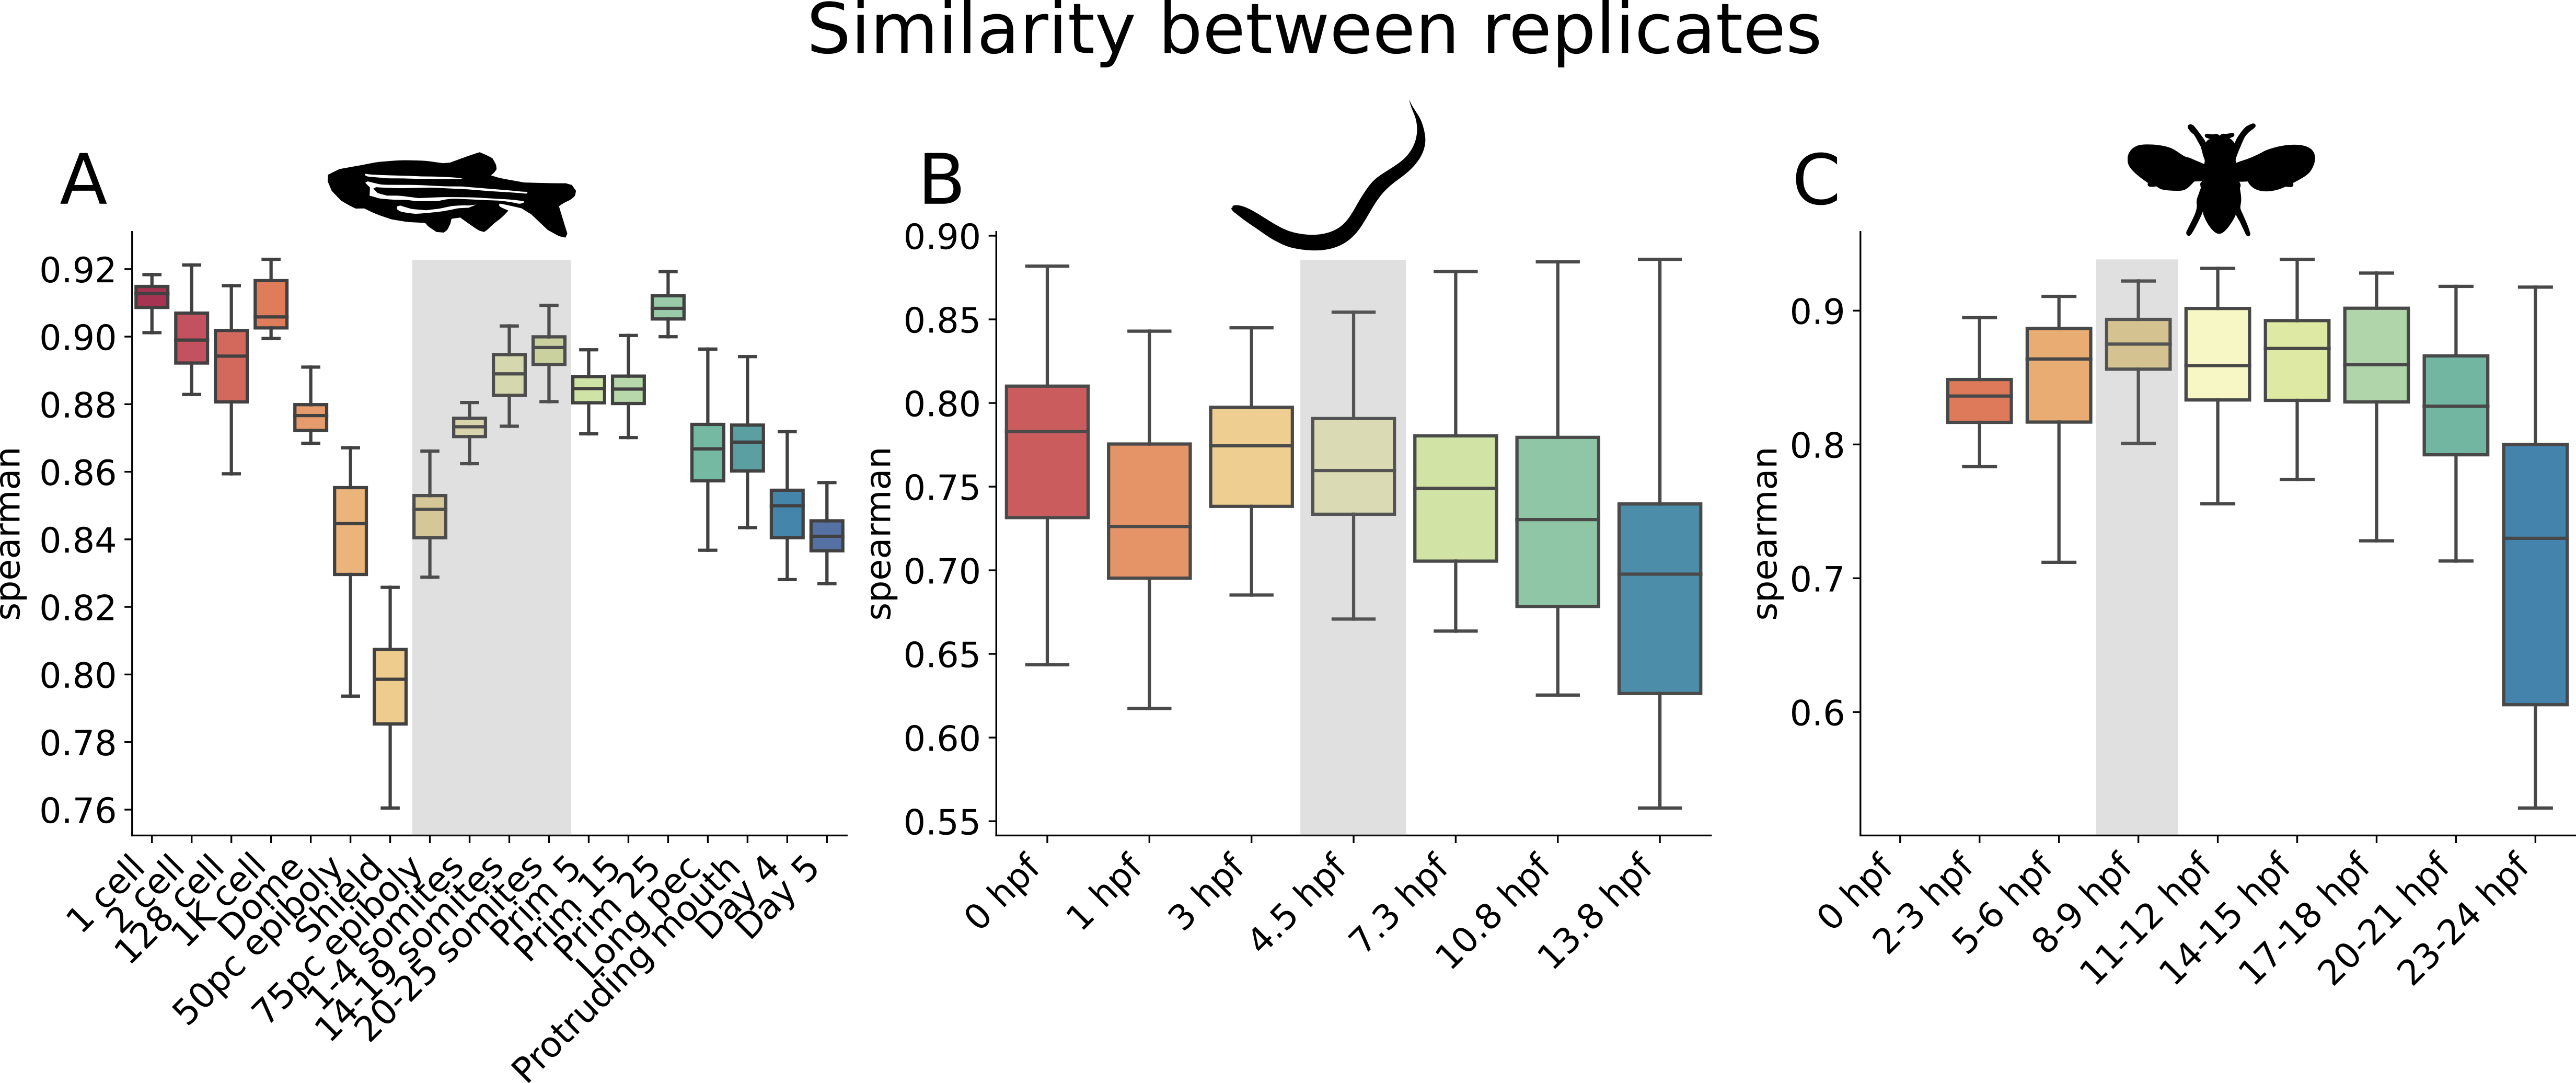
\includegraphics[width=\linewidth]{ch4.hourglass/images/within_timepoint.png}
    \caption{Distribution of gene expression spearman correlation coefficient between replicates belonging to the same stage for (A) single embryo \textit{D. rerio} samples, (B) pools of 10 \textit{C. elegans} embryos, and (C) single-embryo \textit{D. melanogaster} samples. Distribution consists of 250 pairs randomly sampled. The shaded area indicates the phylotypic stage. }
    \label{fig:within_timepoint}
\end{figure}

\begin{figure}[H]
    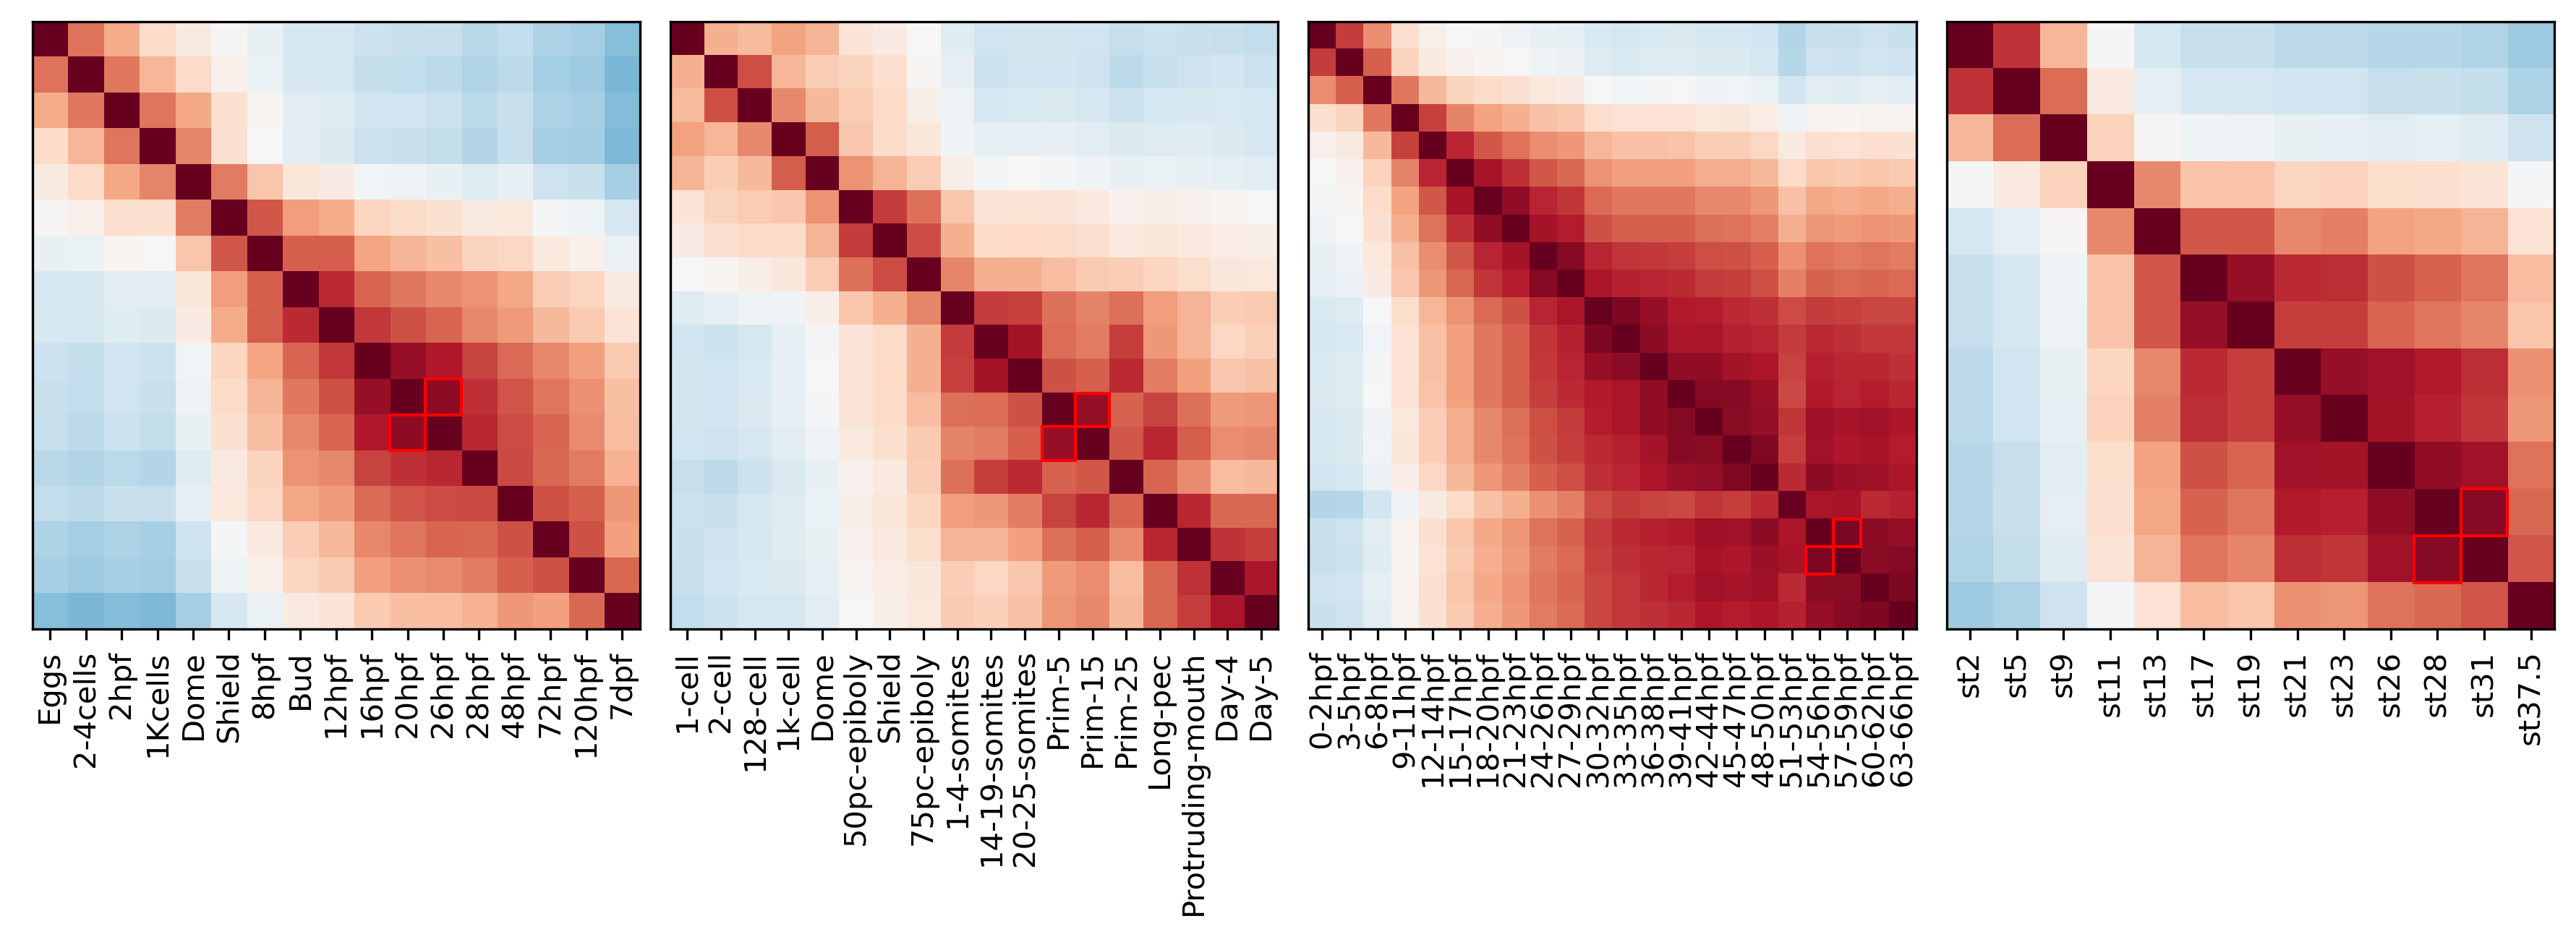
\includegraphics[width=\linewidth]{ch4.hourglass/images/within_species.png}
    \caption{Self-correlation of different}
    \label{fig:withinspecies}
\end{figure}

\begin{figure}[H]
    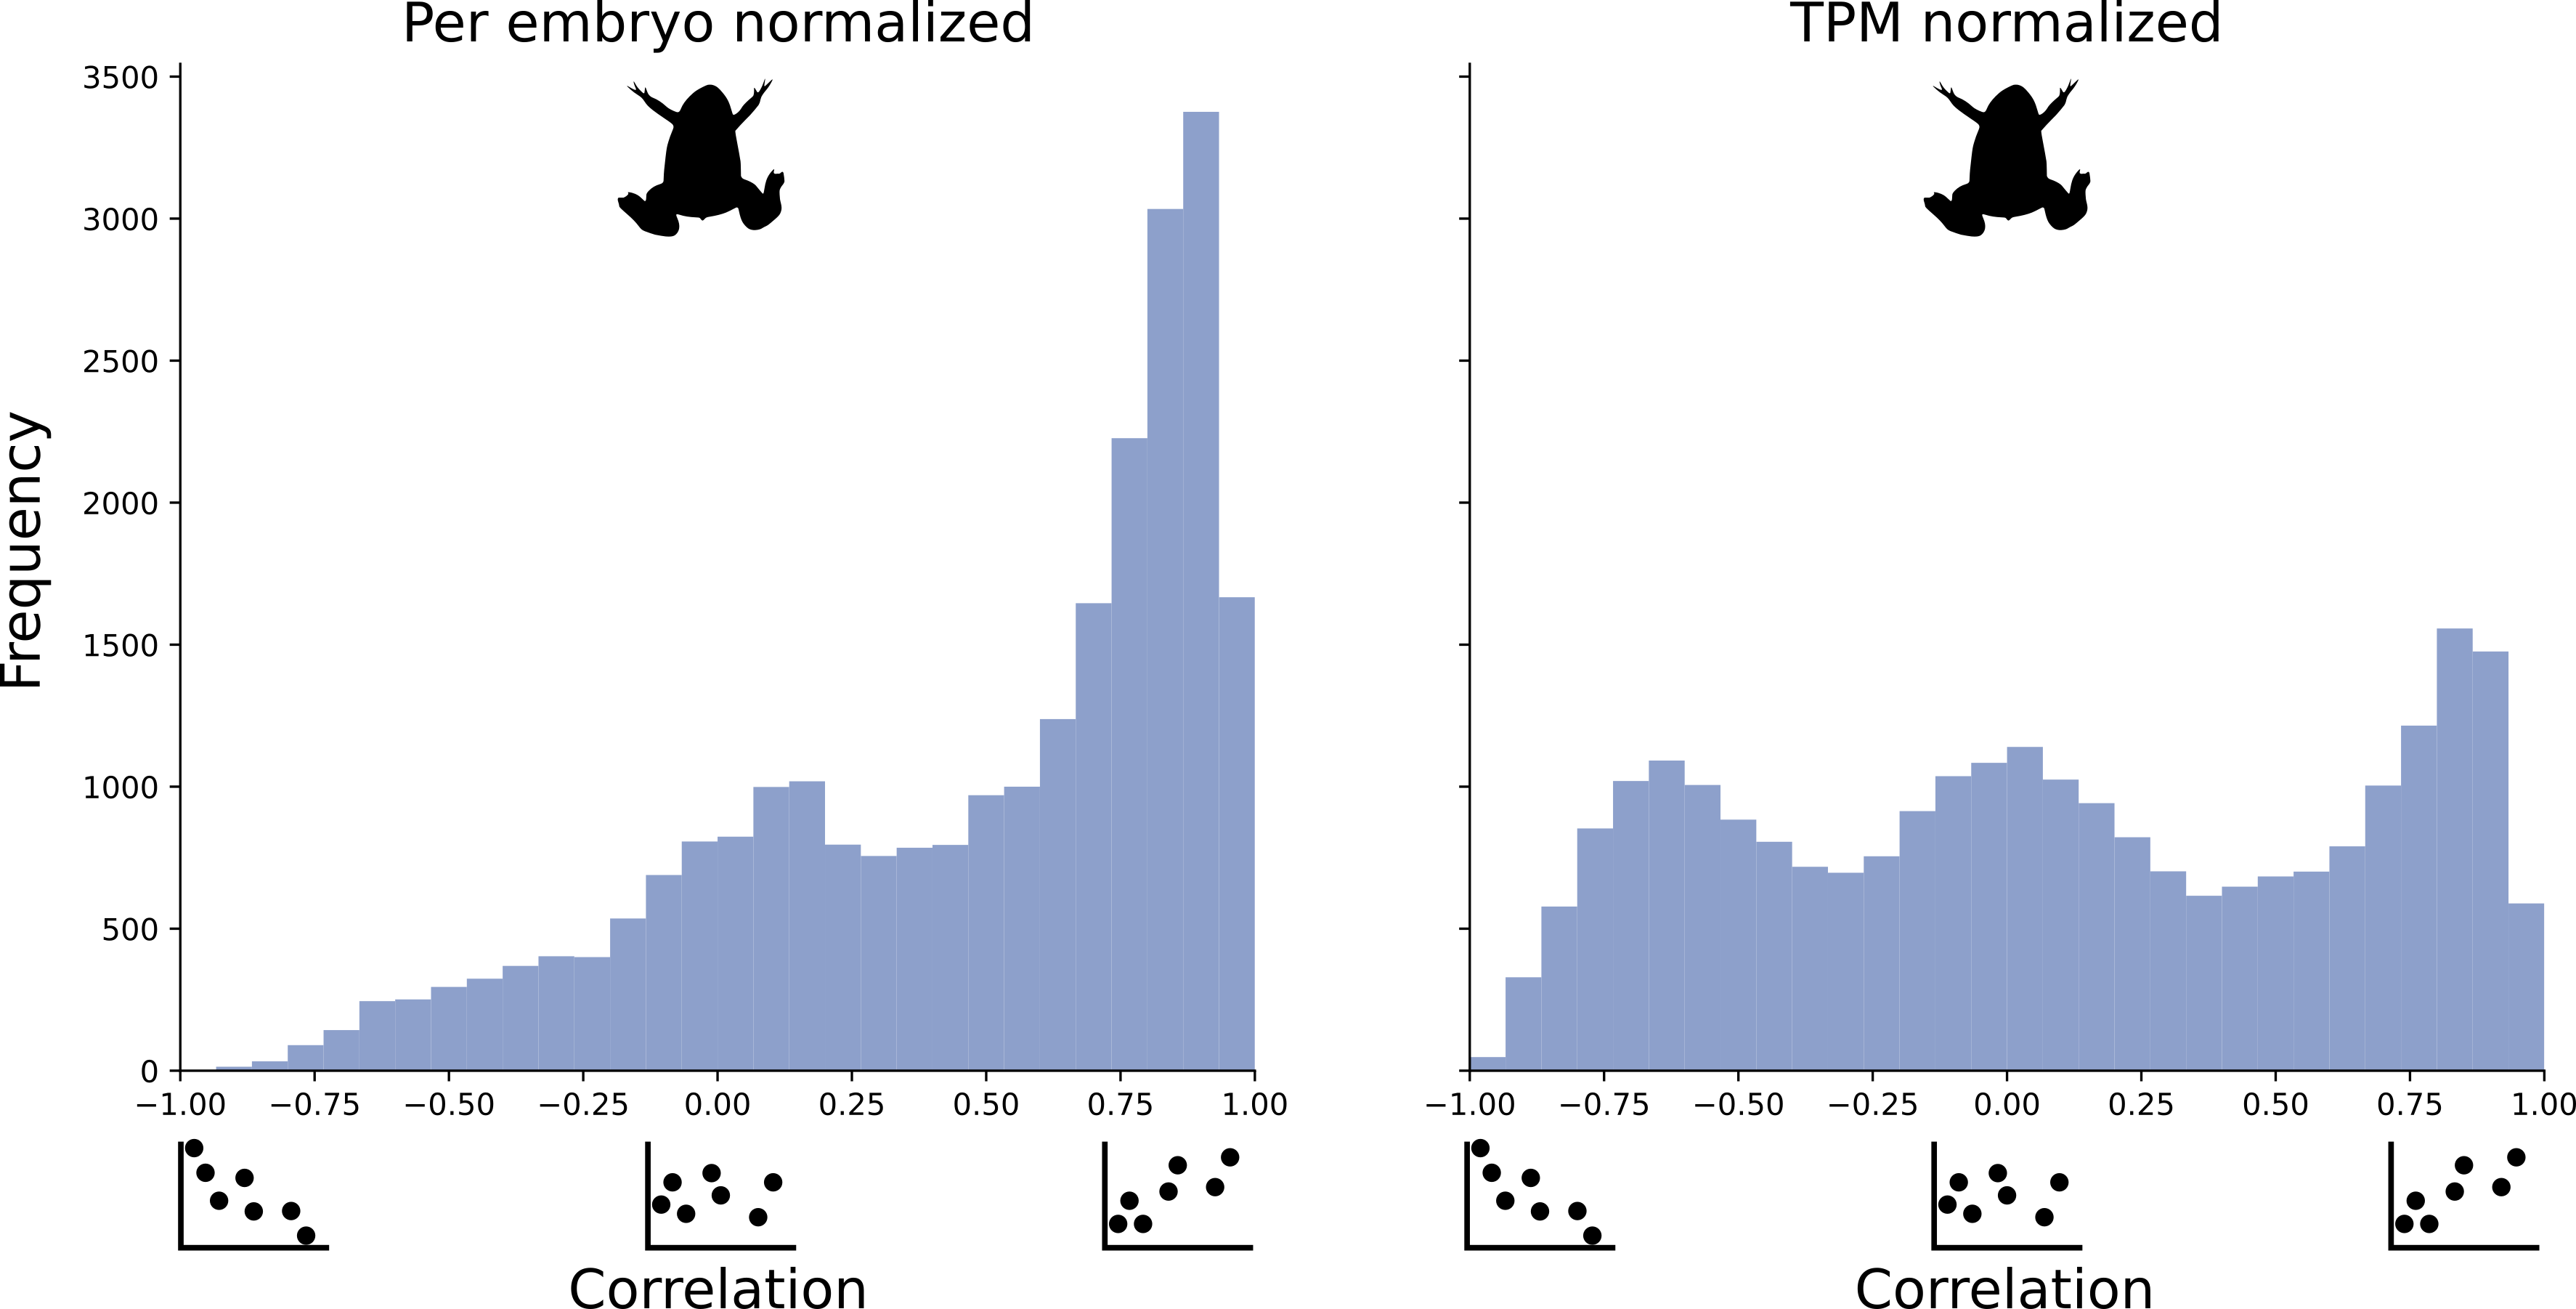
\includegraphics[width=\linewidth]{ch4.hourglass/images/gene_landscape_normalization.png}
    \caption{The difference in gene landscape between per-embryo normalization and TPM normalization of \textit{X. tropicalis}. Figure A shows the gene landscape of per-embryo normalized gene expression. Because the \textit{X. tropicalis} embryo grows practically all genes are upregulated on a per-embryo basis. In panel B the gene landscape of TPM normalized gene expression is visualized. Here we see that there are roughly three groups of gene expression, a down-regulated, a constant, and an up-regulated group. TODO add A and B}
    \label{fig:genelandscapenormalization}
\end{figure}

\begin{figure}[H]
    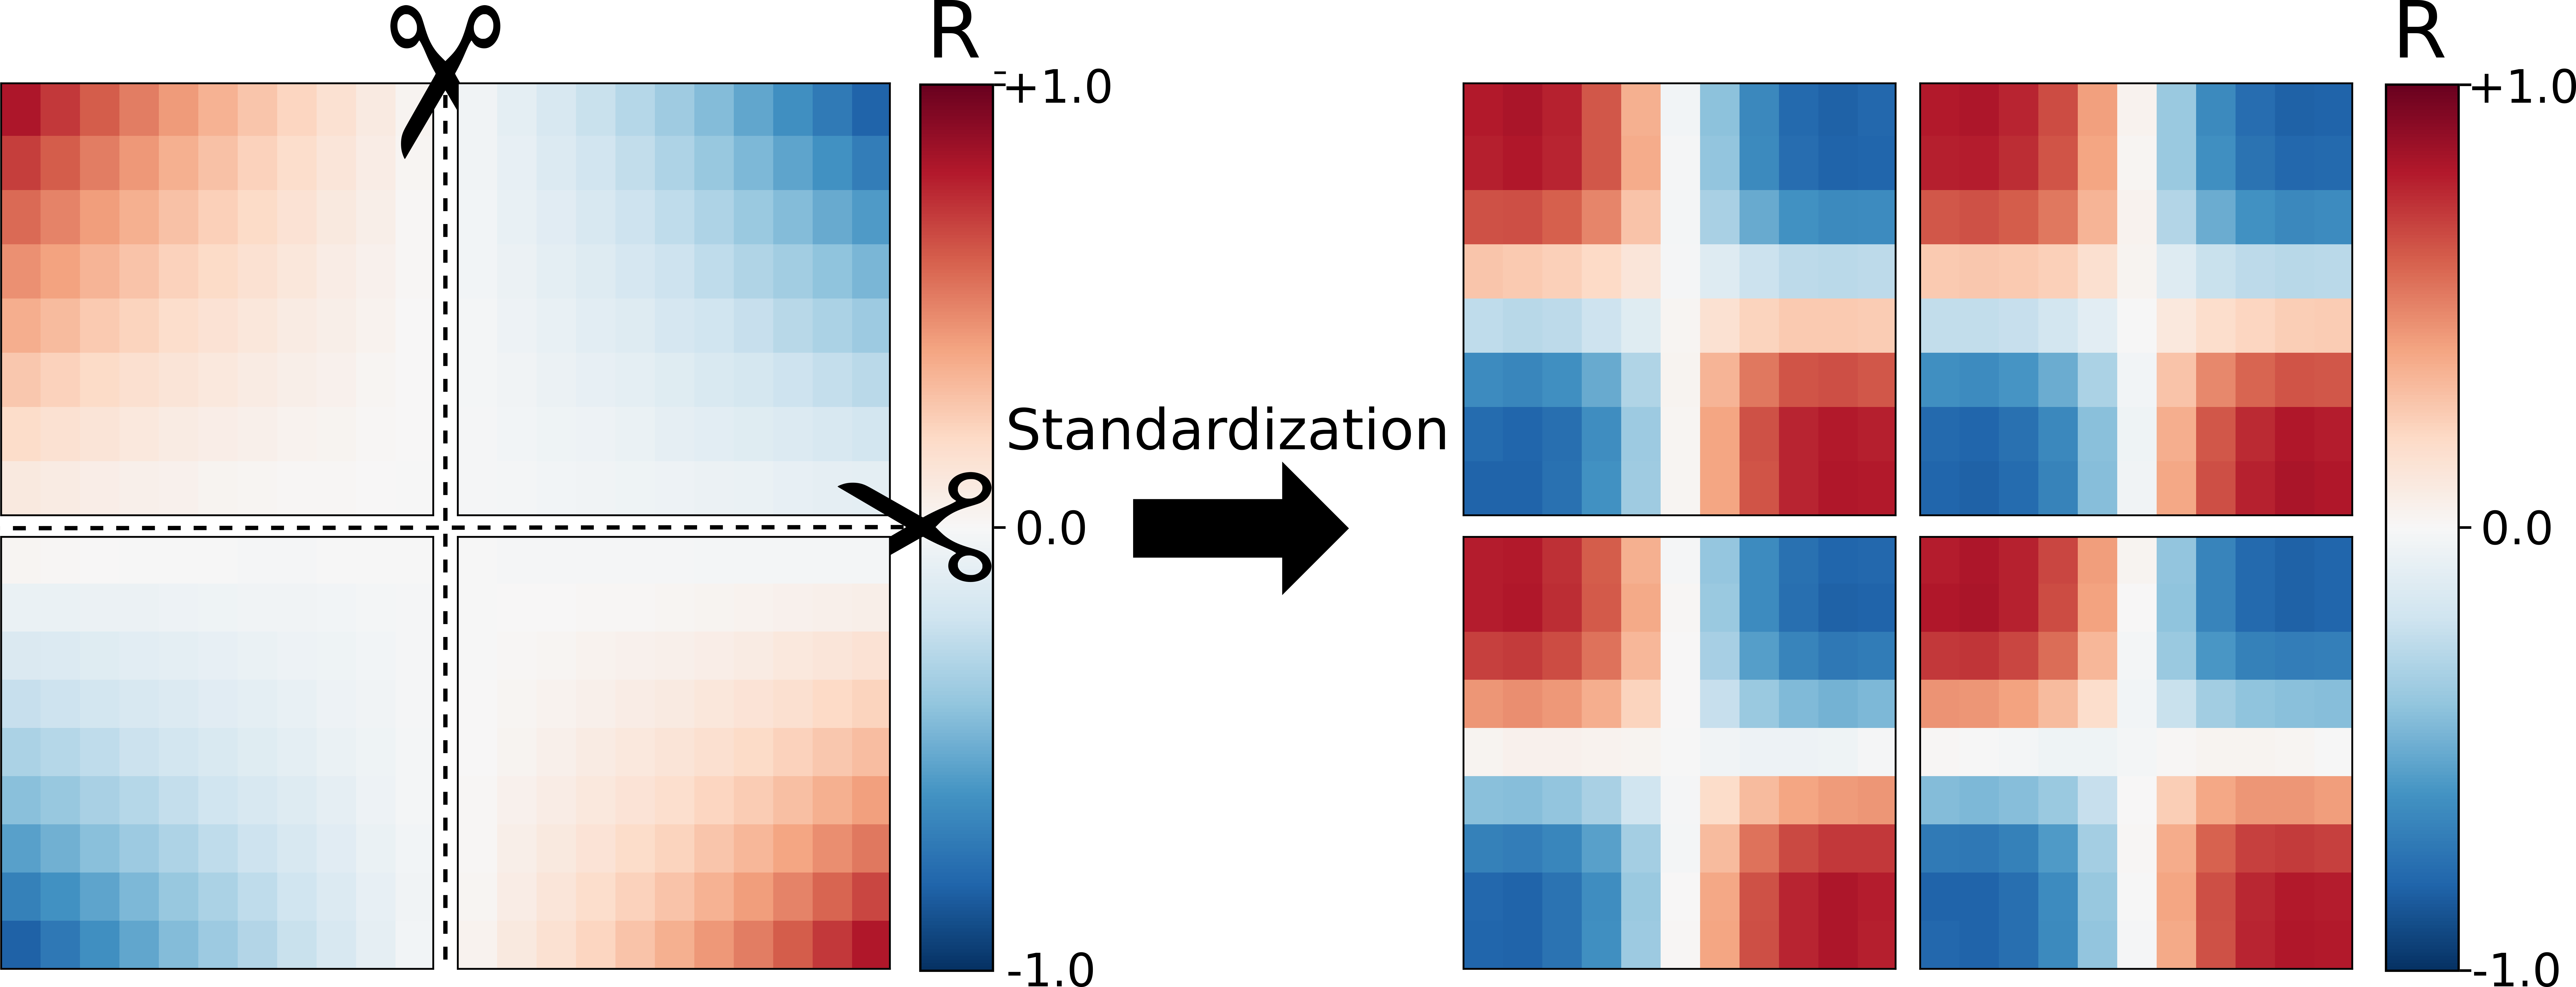
\includegraphics[width=\linewidth]{ch4.hourglass/images/sim_normalisation.png}
    \caption{Cutting the simulated data set into four quarters and applying standardization afterwards results in an inverse hourglass for each quarter.}
    \label{fig:sim_normalisation}
\end{figure}

\begin{figure}[H]
    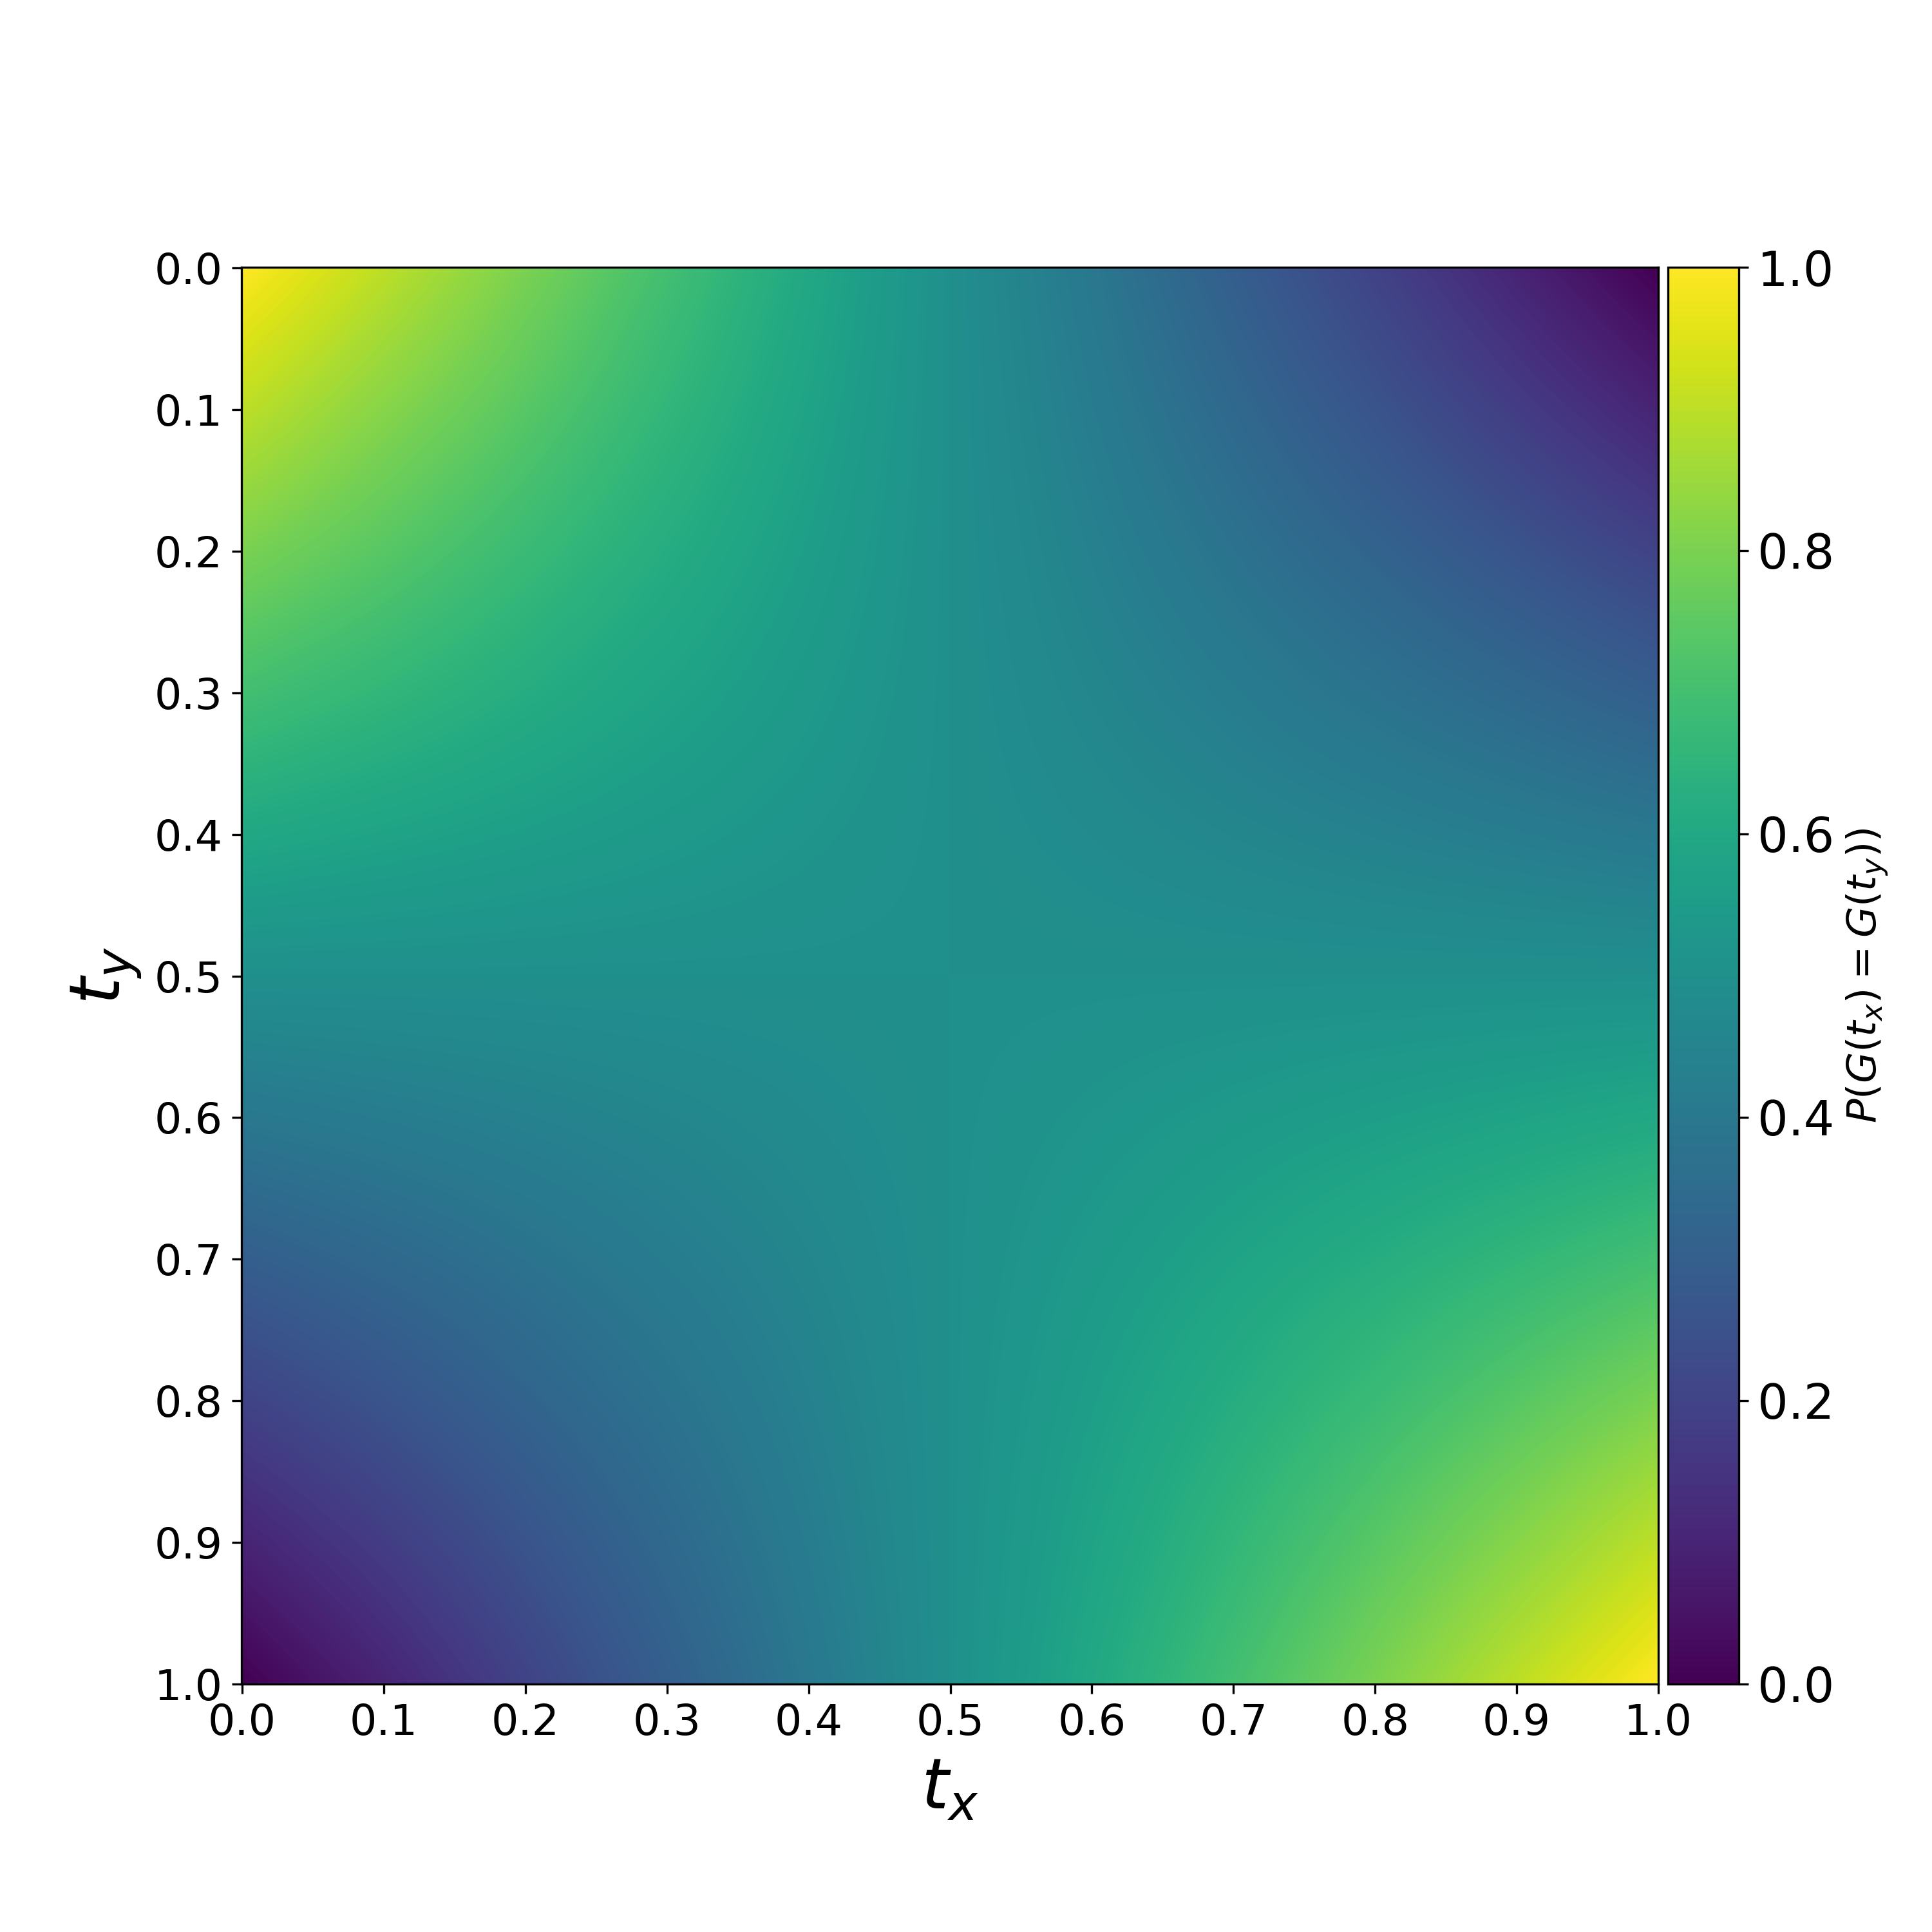
\includegraphics[width=\linewidth]{ch4.hourglass/images/math_inverse.png}
    \caption{The probability that two variables are equal under the assumption that they both start \textit{off} and end \textit{off}, but their moment of switching is random.}
    \label{fig:inverse_math}
\end{figure}

\begin{figure}[H]
    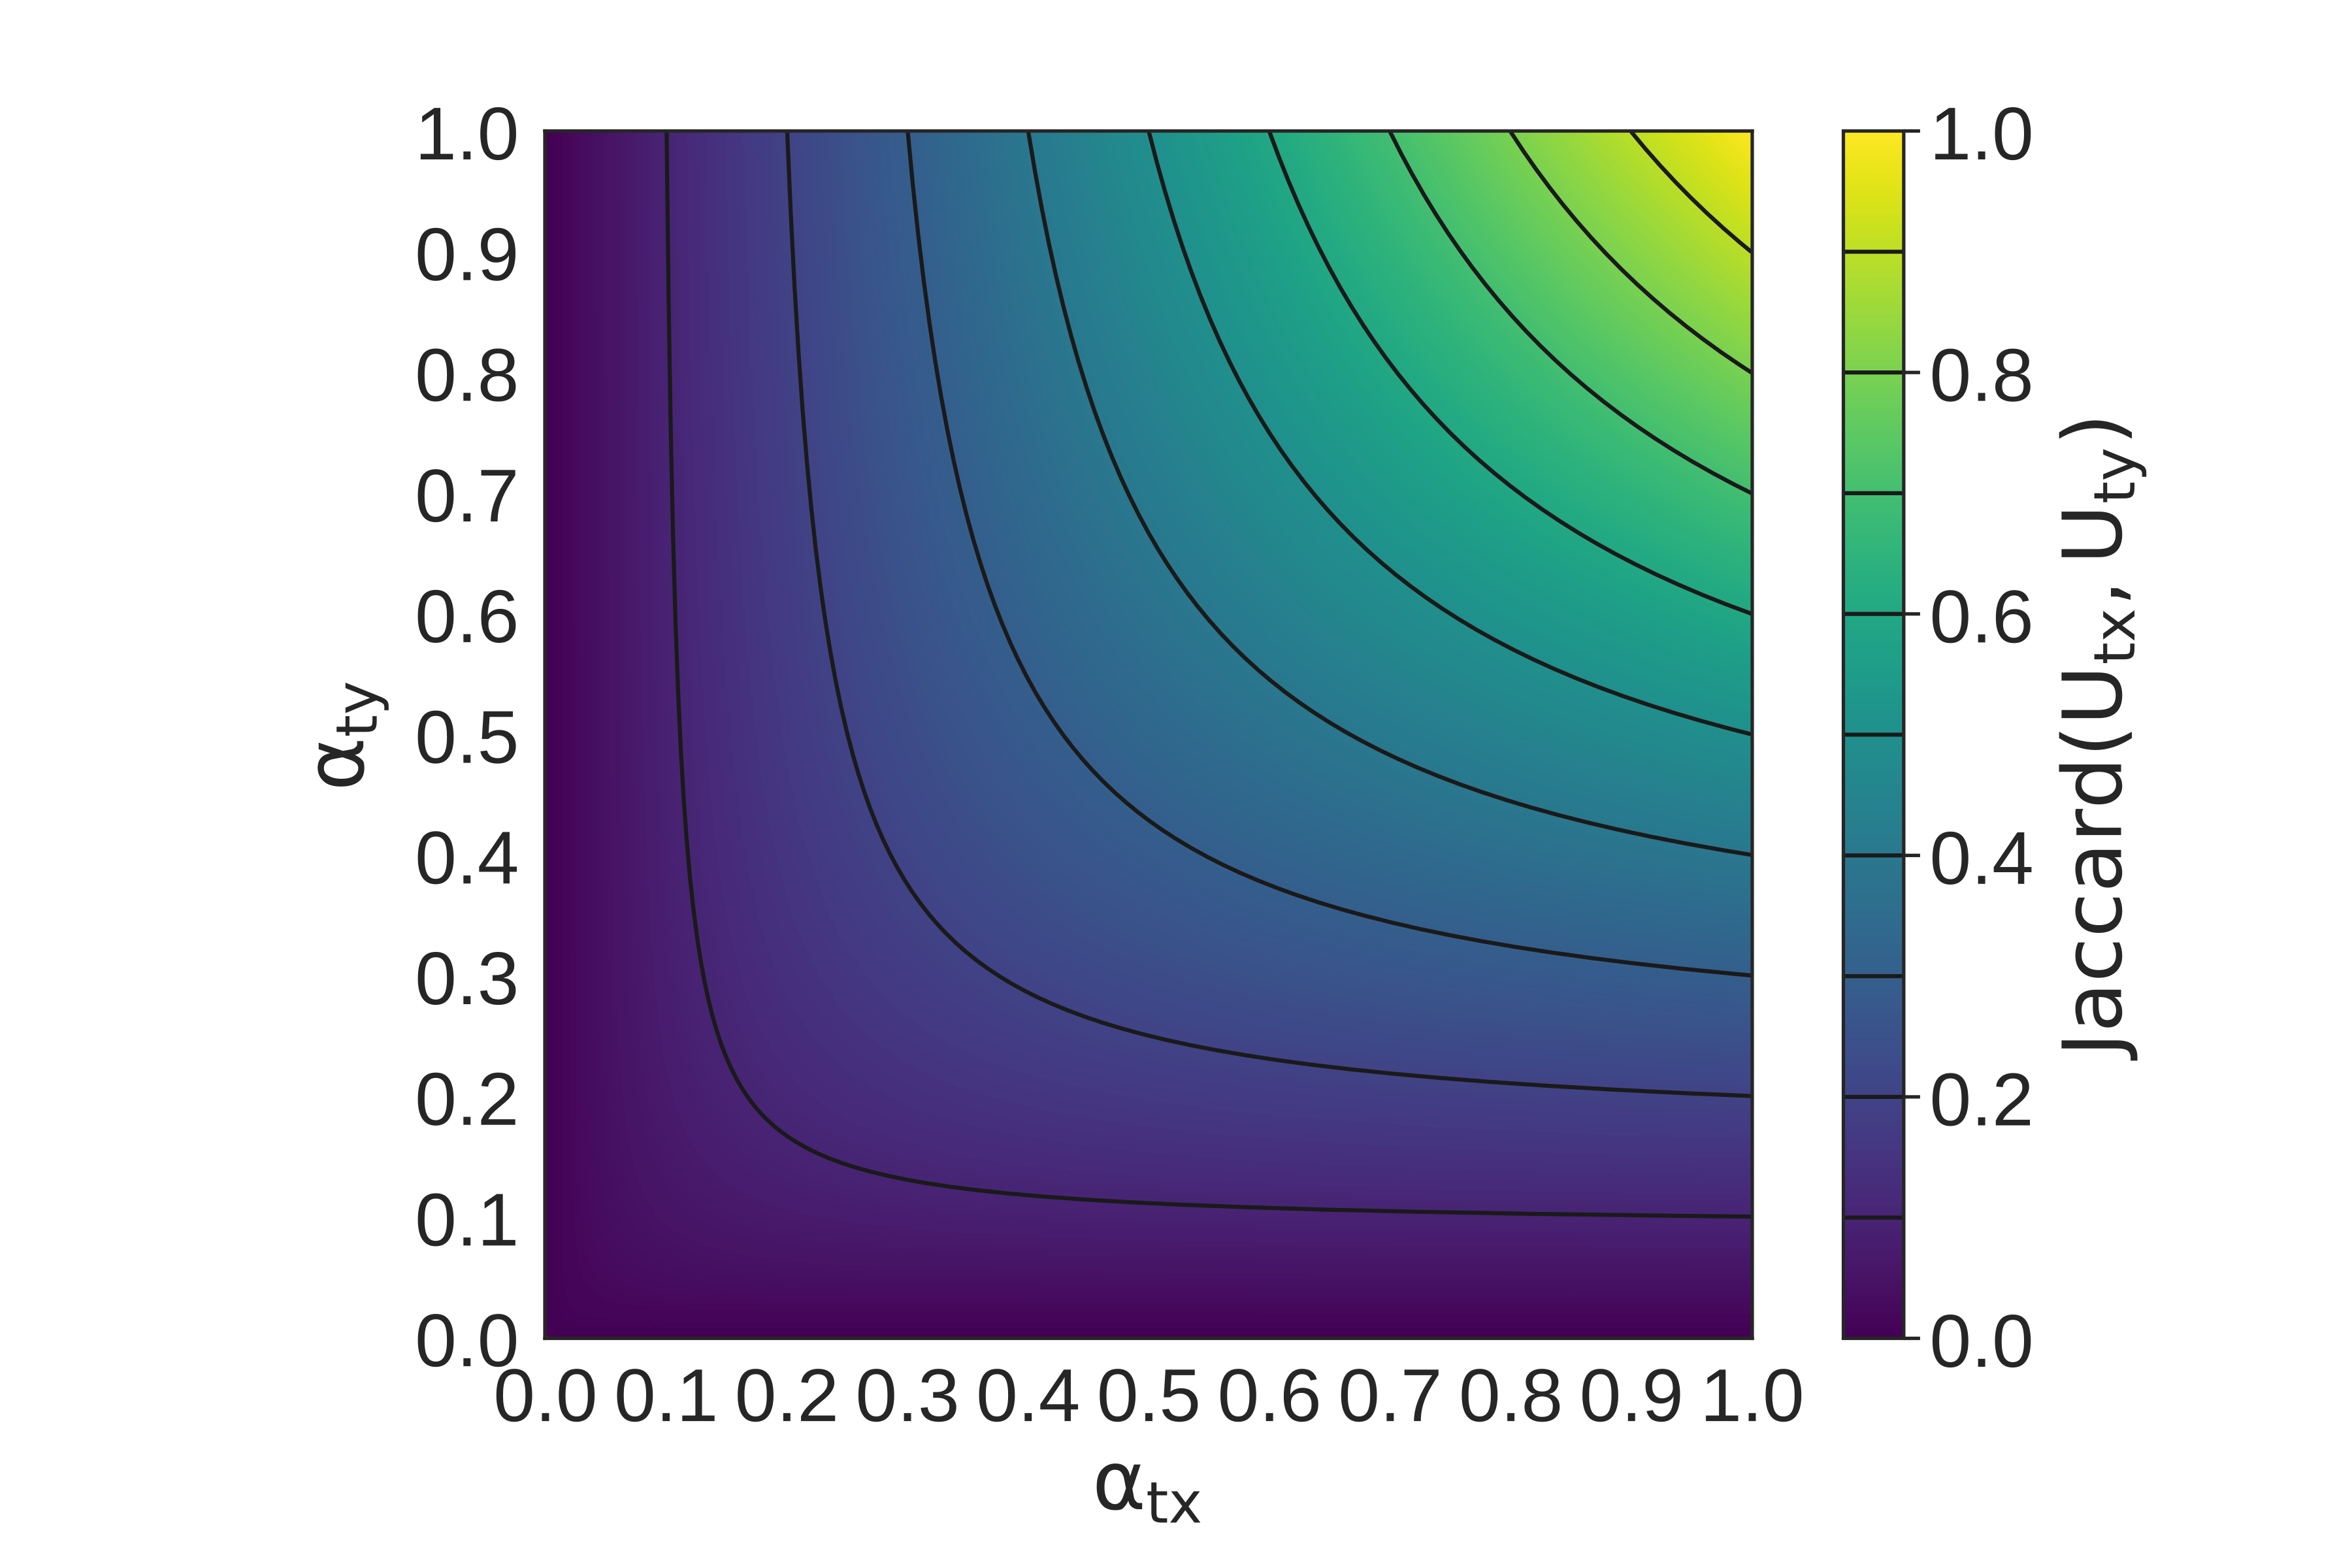
\includegraphics[width=\linewidth]{ch4.hourglass/images/math_flies.png}
    \caption{The Jaccard index landscape.}
    \label{fig:peak_math}
\end{figure}

\begin{figure}[H]
    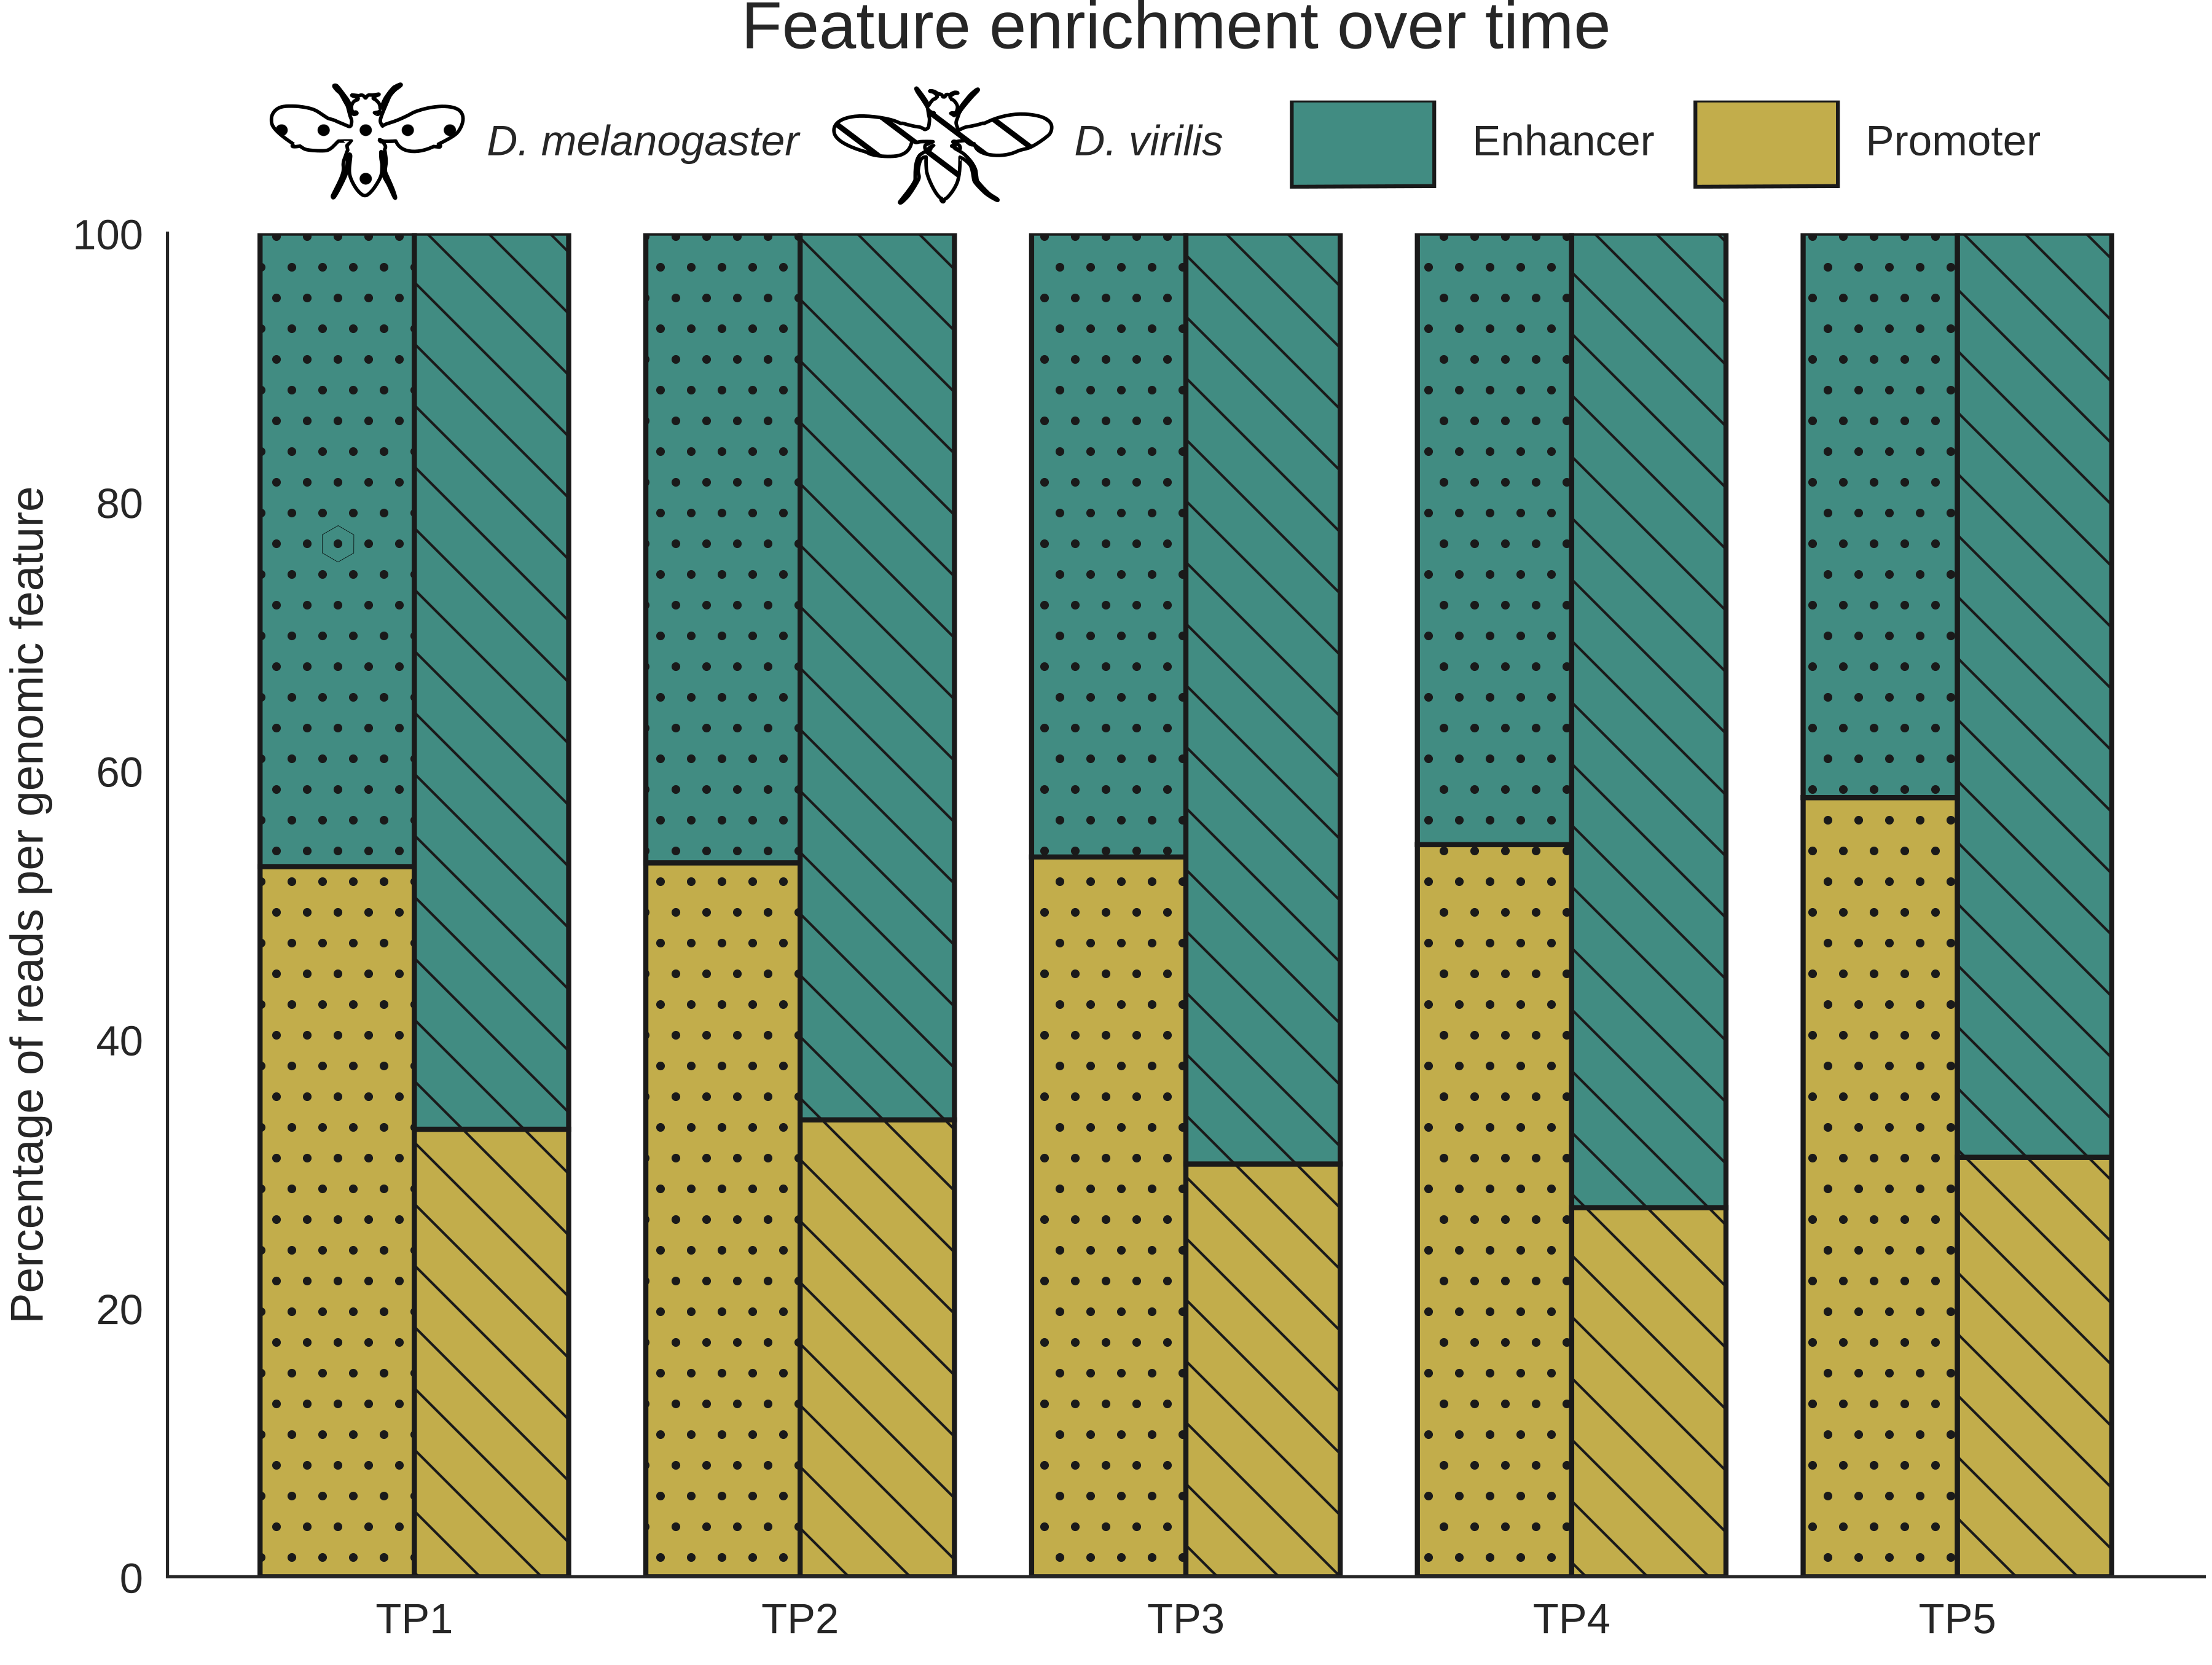
\includegraphics[width=\linewidth]{ch4.hourglass/images/feature_enrichment.png}
    \caption{explain.}
    \label{fig:peak_enrichment}
\end{figure}

\closesupplement
